\begin{enumerate}[label=\thesection.\arabic*,ref=\thesection.\theenumi]

\item  
Find four numbers forming a geometric progression in which the third term is greater than the first term by 9, and the second term is greater than the $4^{th}$ by 18.\\
\solution
\iffalse
\let\negmedspace\undefined
\let\negthickspace\undefined
\documentclass[journal,12pt,onecolumn]{IEEEtran}
\usepackage{cite}
\usepackage{amsmath,amssymb,amsfonts,amsthm}
\usepackage{algorithmic}
\usepackage{graphicx}
\usepackage{textcomp}
\usepackage{xcolor}
\usepackage{txfonts}
\usepackage{listings}
\usepackage{enumitem}
\usepackage{mathtools}
\usepackage{gensymb}
\usepackage{comment}
\usepackage[breaklinks=true]{hyperref}
\usepackage{tkz-euclide} 
\usepackage{listings}
\usepackage{gvv}                                        
\def\inputGnumericTable{}                                 
\usepackage[latin1]{inputenc}                                
\usepackage{color}                                            
\usepackage{array}                                            
\usepackage{longtable}                                       
\usepackage{calc}                                             
\usepackage{multirow}                                         
\usepackage{hhline}                                           
\usepackage{ifthen}                                           
\usepackage{lscape}
\newtheorem{theorem}{Theorem}[section]
\newtheorem{problem}{Problem}
\newtheorem{proposition}{Proposition}[section]
\newtheorem{lemma}{Lemma}[section]
\newtheorem{corollary}[theorem]{Corollary}
\newtheorem{example}{Example}[section]
\newtheorem{definition}[problem]{Definition}
\newcommand{\BEQA}{\begin{eqnarray}}
\newcommand{\EEQA}{\end{eqnarray}}
\newcommand{\define}{\stackrel{\triangle}{=}}
\theoremstyle{remark}
\newtheorem{rem}{Remark}
\begin{document}
\bibliographystyle{IEEEtran}
\vspace{3cm}

\title{NCERT-discrete : 11.9.3 - 21}
\author{EE23BTECH11025 - Anantha Krishnan $^{}$% <-this % stops a space
}
\maketitle
\bigskip

\renewcommand{\thefigure}{\theenumi}
\renewcommand{\thetable}{\theenumi}
\section{question}
Find four numbers forming a geometric progression in which the third term is greater than the first term by 9, and the second term is greater than the $4^{th}$ by 18.\\

\textbf{Solutions :}
\fi
\begin{table}[ht!]
\centering
\begin{tabular}{ |c|c|c| } 
 \hline
Symbols & Description & Values  \\
\hline
 $r$ & Common ratio of the GP & -2\\
 \hline
 $x(n)$ & $(n+1)^{th}$ term of the Sequence & $x(0)r^{n}u(n)$\\
 \hline
 $x(0)$ & First term of the GP & 3\\
\hline
 $x(2)-x(0)$ & First constraint & 9\\
 \hline
 $x(1)-x(3)$& Second constraint & 18\\
 \hline
\end{tabular}
\caption{Parameters, Descriptions, and Values}
\label{table:ee25-tab2}
\end{table}





From the constraints given in \ref{table:ee25-tab2}:
   \begin{align}
x\brak{0}r^2 - 9 &= x\brak{0} \label{eq:ee25-a1}\\
x\brak{0}r + 18 &= x\brak{0}r^3 \label{eq:ee25-a2}\\
\implies x(0)(r^2-1) &= 9 \label{eq:ee25-a3}\\
\implies x (0)r(r^2-1) &=18
\label{eq:ee25-a4}
\end{align}
By dividing $\eqref{eq:ee25-a3}$ and $\eqref{eq:ee25-a4}$ and solving ,we get: 
\begin{align}
    \implies
    x\brak{0} &= 3\\
    \implies
    r &= -2
\end{align}

 Z-Transform for x\brak{n} :
    Using $\eqref{eq:ztrans}$ :
    \begin{align}
    X\brak{z} &= \frac{1}{1+2z^{-1}},\quad \abs {z}>\abs{2} 
    \end{align}
    
    \begin{figure}[!ht]    
    \centering
    \graphicspath{ {ncert-maths/11/9/3/21/figs/} }
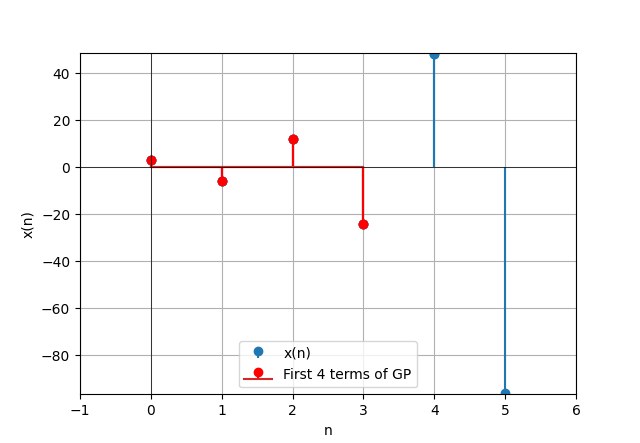
\includegraphics[width=\columnwidth]{graph_1}
\caption{ $x\brak{n}$ vs n }
\label{graph:ee25-ag2}
\end{figure}


\pagebreak

\item The $4^{th}$ term of a G.P. is square of its second term, and the first term is -3. Determine its $7^{th}$ term.\\  

\solution 

\iffalse
\documentclass[journal,12pt,twocolumn]{IEEEtran}
\usepackage{amsmath,amssymb,amsfonts,amsthm}
\usepackage{txfonts}
\usepackage{tkz-euclide}
\usepackage{listings}
\usepackage{gvv}
\usepackage[latin1]{inputenc}
\usepackage{array}
\usepackage{pgf}
\usepackage{lmodern}

\begin{document}
\bibliographystyle{IEEEtran}

\title{DISCRETE 11.9.3 Q-4}
\author{EE23BTECH11066 - Yakkala Amarnath Karthik
}
\maketitle

\bibliographystyle{IEEEtran}
\textbf{Question:} \\ \\The $4^{th}$ term of a G.P. is square of its second term, and the first term is -3. Determine its $7^{th}$ term.\\ \\
\textbf{Solution:}
\fi
\begin{table}[h!]
  \centering
    \begin{tabular}{|c|c|c|}
    \hline
    \textbf{Variable} & \textbf{Description} & \textbf{value}\\
    \hline
    $x(0)$ & first term of G.P. & -3 \\
    \hline
    $r$ & Common ratio of G.P. & ? \\
    \hline
    $x(n)$ & general term of the G.P. & $x\brak0r^{n}$ \\
    \hline
    $x\brak3$ & fourth term & $\sbrak{x\brak1}^2$\\
    \hline
    $u\brak{n}$ & unit step function & - \\
    \hline
  \end{tabular}

  \caption{A Table with input parameters}
  \label{tab:11.9.3.4.1}
\end{table}
from \tabref{tab:11.9.3.4.1}
\begin{align}
 x\brak0r^{3}&=\brak{x\brak0r^{1}}^2\\
 &=x\brak0^2r^2\\
\implies r&=x\brak0\\
&=-3
\end{align}
general term
\begin{align}
x\brak{n}&=x\brak0r^nu\brak{n}\\
&=\brak{-3}^{n+1}u\brak{n}
\end{align}
The $7^{th}$ term of the sequence will be:
\begin{align}
x\brak6 & =\brak{-3}\brak{-3}^{6}\\
& =-2187
\end{align}
Z transform of the given G.P is:
\begin{align}
X\brak{z}=\frac{x\brak0}{1-rz^{-1}}= \frac{-3}{1+3z^{-1}}.\hspace{0.5cm} |z|>3
\end{align}
\bigskip
\begin{figure}[ht]
        \centering
        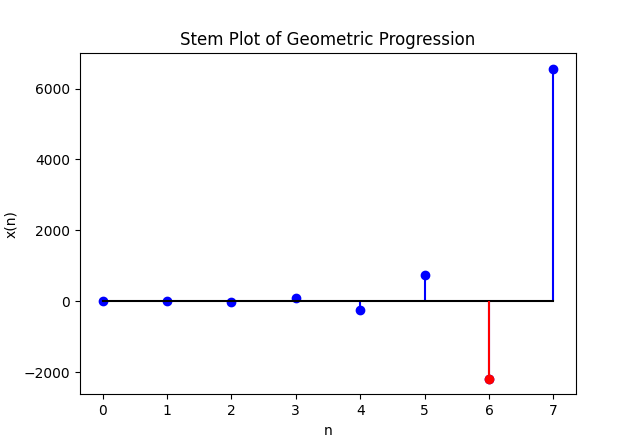
\includegraphics[width=0.45\textwidth]{ncert-maths/11/9/3/4/figs/stemplotfinal.jpeg}
        \caption{Graph showing first 8 terms of the GP}
    \end{figure} \\
%\end{document}

\pagebreak

\item Show that
\begin{equation}
    \frac{1\times2^2 + 2\times3^2 + \dots + n\times\brak{n+1}^2}{1^2\times2 + 2^2\times3 +\dots + n^2\times\brak{n+1}}  = \frac{3n+5}{3n+1}\notag
\end{equation}

\solution 

\iffalse
\let\negmedspace\undefined
\let\negthickspace\undefined
\documentclass[journal,12pt,twocolumn]{IEEEtran}
\usepackage{cite}
\usepackage{amsmath,enumitem,amssymb,amsfonts,amsthm}
\usepackage{algorithmic}
\usepackage{graphicx}
\usepackage{float}
\usepackage{textcomp}
\usepackage{xcolor}
\usepackage{caption}
\usepackage{txfonts}
\usepackage{listings}
\usepackage{enumitem}
\usepackage{mathtools}
\usepackage{gensymb}
\usepackage{comment}
\usepackage[breaklinks=true]{hyperref} 
\usepackage{tkz-euclide} 
\usepackage{listings}
\usepackage{tabularx}
\usepackage{gvv}                                        
\def\inputGnumericTable{}                                 
\usepackage[latin1]{inputenc}                              
\usepackage{color}                                            
\usepackage{array}                                            
\usepackage{longtable}                                       
\usepackage{calc}                                             
\usepackage{multirow}                                         
\usepackage{hhline}                                           
\usepackage{ifthen}                                        
\usepackage{lscape}
\newtheorem{theorem}{Theorem}[section]
\newtheorem{problem}{Problem}
\newtheorem{proposition}{Proposition}[section]
\newtheorem{lemma}{Lemma}[section]
\newtheorem{corollary}[theorem]{Corollary}
\newtheorem{example}{Example}[section]
\newtheorem{definition}[problem]{Definition}
\newcommand{\BEQA}{\begin{eqnarray}}
\newcommand{\EEQA}{\end{eqnarray}}
\newcommand{\define}{\stackrel{\triangle}{=}}
\theoremstyle{remark}
\newtheorem{rem}{Remark}
\begin{document}
\bibliographystyle{IEEEtran}
\vspace{3cm}
\title{NCERT 11.9.5 26Q}
\author{EE23BTECH11015 - DHANUSH V NAYAK$^{*}$% <-this % stops a space
}
\maketitle
\newpage
\bigskip
\renewcommand{\thefigure}{\arabic{figure}}
\renewcommand{\thetable}{\theenumi}
\bibliographystyle{IEEEtran}
\textbf{\underline{RESULTS AND DERIVATIONS}}

\newpage
\textbf{Question:} Show that
\begin{equation}
    \frac{1\times2^2 + 2\times3^2 + \dots + n\times\brak{n+1}^2}{1^2\times2 + 2^2\times3 +\dots + n^2\times\brak{n+1}}  = \frac{3n+5}{3n+1}\notag
\end{equation}
\textbf{Solution:}
\fi 

\begin{table}[h]
    \centering
    \renewcommand\thetable{1}
    \setlength{\extrarowheight}{9pt}
    \resizebox{0.54\textwidth}{!}{
    \begin{tabular}{|c|c|c|}
    \hline
    \textbf{Parameter} & \textbf{Description} & \textbf{Value} \\ \hline
    $n$ & Integer &.... -2,-1,0,1, 2, ... \\ \hline
    $x_1(n)$ & General term of Numerator & $\vphantom{\brak{n^{3}}} \brak{n^{3} + 5n^{2} + 8n + 4} \cdot u\brak{n}$ \\ \hline
    $x_2(n)$ & General Term of Denominator  & $\vphantom{\brak{n^{3}}} \brak{n^{3}+4n^{2}+5n+2}\cdot u\brak{n}$ \\ \hline
    $y_1\brak{n}$ & Sum of terms of numerator & $?$ \\ \hline
    $y_2\brak{n}$ & Sum of terms of denominator & $? $ \\ \hline
    $U(z)$ & z-transform of $u(n)$ & $\frac{1}{1 - z^{-1}\vphantom {\brak{0.3pt}}},\cbrak{z\in\mathbb{C} : \lvert z \rvert > 1}$ \\ \hline 
    ROC & Region of convergence & $\left\{ z : \left|\sum_{n=-\infty}^{\infty} x(n)z^{-n}\right| < \infty \vphantom {\brak{{0.3pt}}}\right\}$ \\ \hline 
    \end{tabular}}
    \caption{Parameter Table}
    \label{tab:11.9.5.26.1}
    \end{table}
    
    
    
    
\begin{enumerate}[label=\arabic*.]
\item \underline {Analysis of Numerator:}\\
\begin{align}
 X_1\brak{z} &= \sum_{n=-\infty}^\infty x_1\brak{n}  z^{-n}\\
             &= \sum_{n=-\infty}^\infty \brak{n^{3} + 5n^{2} + 8n + 4} u\brak{n} z^{-n}
\end{align}
Using results of equations \eqref{eq:11.9.5.26.2} to \eqref{eq:11.9.5.26.5} we get:
\begin{align}
 \therefore   X_1\brak{z}&= \frac{4+2z^{-1}}{\brak{1-z^{-1}}^4} ,   \abs{z} >1 
\end{align}
From \eqref{eq:conv-sum}
\begin{align}
y_1\brak{n} &= x_1\brak{n}\ast u\brak{n}\\
    Y_1\brak{z} &= X_1\brak{z} U\brak{z} \\
 &= \frac{4+2z^{-1}}{\brak{1-z^{-1}}^5} , \abs{z}> 1 
\end{align}
Using partial fractions:
\begin{align}
    Y_1(z) &= \frac{22z^{-1}}{\brak{1-z^{-1}}} + \frac{48z^{-2}}{\brak{1-z^{-1}}^2} + \frac{52z^{-3}}{\brak{1-z^{-3}}^3} , \label{eq:11.9.5.26.6}\\
    &+ \frac{28z^{-4}}{\brak{1-z^{-1}}^4}+\frac{6z^{-5}}{\brak{1-z^{-1}}^5}+4 , \abs{z}>1 \notag 
\end{align}
Substituting results of equation \eqref{eq:11.9.5.26.9} to \eqref{eq:11.9.5.26.12} in equation \eqref{eq:11.9.5.26.6}:
\begin{align}
    y_1\brak{n} &= \frac{3n^4 + 26n^3 + 81n^2 + 106n + 48}{12}u\brak{n}\\
    &= \frac{\brak{3n+8}\brak{n+1}\brak{n+2}\brak{n+3}}{12}u\brak{n}
\end{align}
\item \underline{Analysis of Denominator:}
\begin{align}
    X_2\brak{z} &= \sum_{n=-\infty}^\infty x_2\brak{n} z^{-n}\\
                &= \sum_{n=-\infty}^\infty \brak{n^{3}+4n^{2}+5n+2} u\brak{n} z^{-n}
\end{align}
\text{Using results of equation \eqref{eq:11.9.5.26.2} to \eqref{eq:11.9.5.26.5} we get:}
\begin{align}
   \therefore  X_2\brak{z} &= \frac{2+4z^{-1}}{\brak{1-z^{-1}}^4},   \abs{z} >1   
\end{align}
From \eqref{eq:conv-sum}
\begin{align}
    y_2\brak{n} &= x_2\brak{n}\ast u\brak{n}\\
    Y_2\brak{z} &= X_2\brak{z} U\brak{z} \\
 &=\frac{2+4z^{-1}}{\brak{1-z^{-1}}^5} ,   \abs{z} >1 
\end{align}
Using partial fractions:
\begin{align}
    Y_2\brak{z} &= \frac{14z^{-1}}{\brak{1-z^{-1}}} + \frac{36z^{-2}}{\brak{1-z^{-1}}^2} + \frac{44z^{-3}}{\brak{1-z^{-3}}^3} \label{eq:11.9.5.26.13}\\
    &+ \frac{26z^{-4}}{\brak{1-z^{-1}}^4}+\frac{6z^{-5}}{\brak{1-z^{-1}}^5}+2 , \abs{z}>1\notag 
\end{align}
Substituting results of equation \eqref{eq:11.9.5.26.9} to \eqref{eq:11.9.5.26.12} in equation \eqref{eq:11.9.5.26.13}:
\begin{align}
    y_2\brak{n} &=  \frac{3n^4 + 22n^3 + 57n^2 + 62n + 24}{12}u\brak{n}\\
                &= \frac{\brak{3n+4}\brak{n+1}\brak{n+2}\brak{n+3}}{12}u\brak{n}
\end{align}
As the sequence start from $n=0$ , in RHS of question $n$ should be replaced by $n+1$:
\begin{align}
    \frac{y_1\brak{n}}{y_2\brak{n}} = \frac{3n+8}{3n+4}
\end{align}
Hence Prooved.
\end{enumerate}
\begin{figure}[htbp]
    \centering
    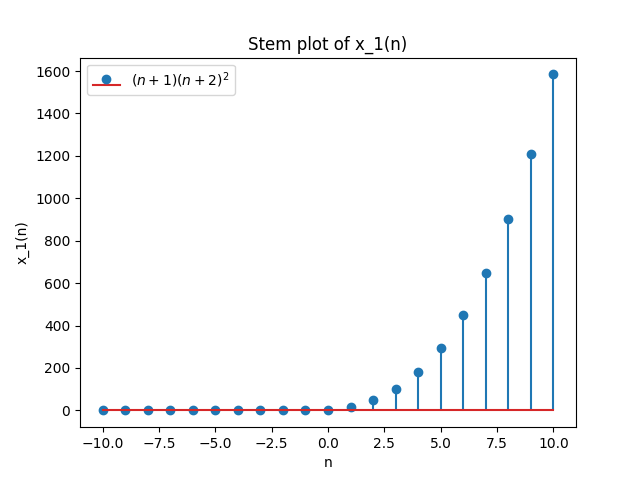
\includegraphics[width=1\columnwidth]{ncert-maths/11/9/5/26/figs/x1_plot.png}
    \caption{Stem Plot of $x_1\brak{n}$}
    \label{fig:x1}
\end{figure}
\begin{figure}[htbp]
    \centering
    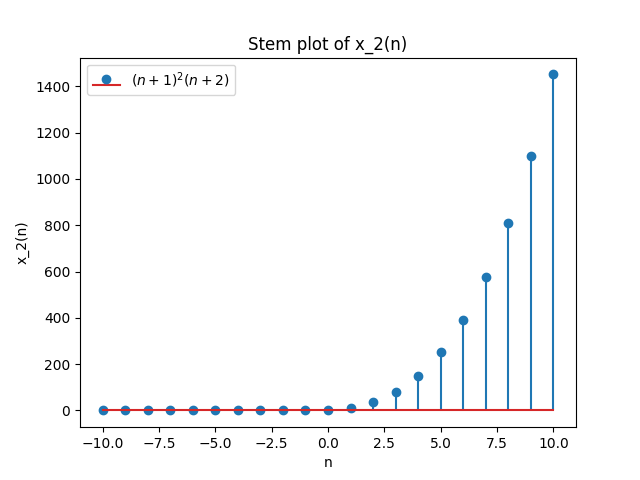
\includegraphics[width=1\columnwidth]{ncert-maths/11/9/5/26/figs/x2_plot.png}
    \caption{Stem Plot of $x_2\brak{n}$}
    \label{fig:x2}
\end{figure}
\begin{figure}[htbp]
    \centering
    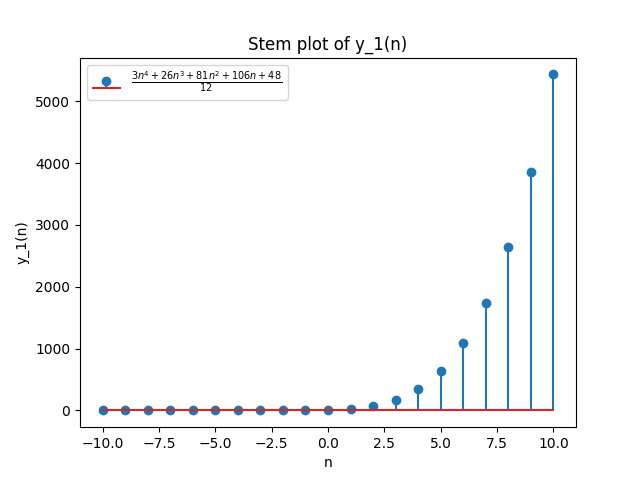
\includegraphics[width=1\columnwidth]{ncert-maths/11/9/5/26/figs/y1_plot.png}
    \caption{Stem Plot of $y_1\brak{n}$}
    \label{fig:y1}
\end{figure}
\begin{figure}[h]
    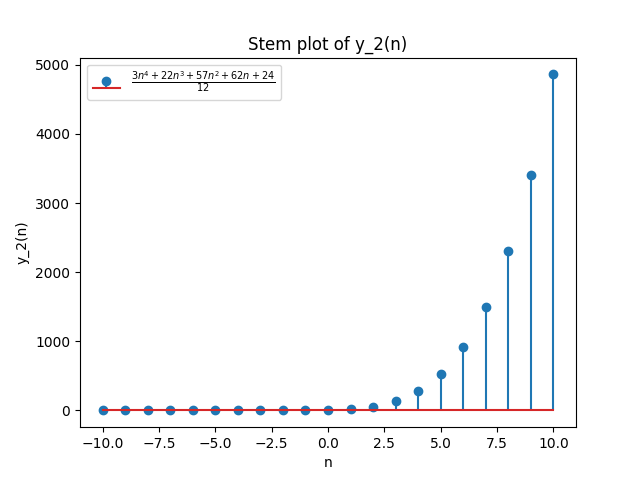
\includegraphics[width=1\columnwidth]{ncert-maths/11/9/5/26/figs/y2_plot.png}
    \caption{Stem Plot of $y_2\brak{n}$}
    \label{fig:y2}
\end{figure}
%\end{document}

\pagebreak

\item Write the five terms at n = 1, 2, 3, 4, 5 of the sequence and obtain the Z-transform of the series
\begin{align}
    x \brak{n} &=  -1, & n = 0 \\
    &=   \frac{x \brak{n-1}}{n}, & n > 0\\
    &=   0, & n < 0 
\end{align}

\solution

\iffalse
\let\negmedspace\undefined
\let\negthickspace\undefined
\documentclass[journal,12pt,twocolumn]{IEEEtran}
\usepackage{cite}
\usepackage{amsmath,amssymb,amsfonts}
\usepackage{graphicx}
\usepackage{textcomp}
\usepackage{xcolor}
\usepackage{txfonts}
\usepackage{listings}
\usepackage{enumitem}
\usepackage{mathtools}
\usepackage{gensymb}
\usepackage{comment}
\usepackage[breaklinks=true]{hyperref}
\usepackage{tkz-euclide} 
\usepackage{listings}
\usepackage{gvv}                                        
\def\inputGnumericTable{}                                 
\usepackage[latin1]{inputenc}                                
\usepackage{color}                                            
\usepackage{array}                                            
\usepackage{longtable}                                       
\usepackage{calc}                                             
\usepackage{multirow}                                         
\usepackage{hhline}                                           
\usepackage{ifthen}                                           
\usepackage{lscape}
\usepackage[export]{adjustbox}

\newtheorem{theorem}{Theorem}[section]
\newtheorem{problem}{Problem}
\newtheorem{proposition}{Proposition}[section]
\newtheorem{lemma}{Lemma}[section]
\newtheorem{corollary}[theorem]{Corollary}
\newtheorem{example}{Example}[section]
\newtheorem{definition}[problem]{Definition}
\newcommand{\BEQA}{\begin{eqnarray}}
\newcommand{\EEQA}{\end{eqnarray}}
\newcommand{\define}{\stackrel{\triangle}{=}}
\newtheorem{rem}{Remark}

\begin{document}
\parindent 0px
\bibliographystyle{IEEEtran}

\vspace{3cm}

\title{}
\author{EE23BTECH11217 - Prajwal M$^{*}$
}
\maketitle
\newpage
\bigskip

 \renewcommand{\thefigure}{\theenumi}
 \renewcommand{\thetable}{\theenumi}


\section*{Exercise 9.1}

\noindent \textbf{12} \hspace{2pt}Write the five terms at n = 1, 2, 3, 4, 5 of the sequence and obtain the Z-transform of the series
\begin{align}
    x \brak{n} &=  -1, & n = 0 \\
    &=   \frac{x \brak{n-1}}{n}, & n > 0\\
    &=   0, & n < 0 
\end{align}

\noindent Solution:
\fi
\noindent
\begin{align}
	x \brak{1} & = \frac{x \brak{0}}{1} = -1 \\
x \brak{2} & = \frac{x \brak{1}}{2} = -\frac{1}{2} \\
	x \brak{3} & = \frac{x \brak{2}}{3} = -\frac{1}{\brak{2} \brak{3}} = -\frac{1}{6}\\
	x \brak{4} & = \frac{x \brak{3}}{4} = -\frac{1}{\brak{2}   \brak{3} \brak{4}} = -\frac{1}{24}\\
	x \brak{5} & = \frac{x \brak{4}}{5} = -\frac{1}{\brak{2} \brak{3} \brak{4} \brak{5}} = -\frac{1}{120} \\
    x \brak{n} & = \frac{-1}{n!}  \brak{u \brak{n}} \label{x(n)}
\end{align}
\begin{align}
	x \brak{n} & \system{Z} X \brak{z} 
\end{align}

\begin{figure}[h]
   \centering
   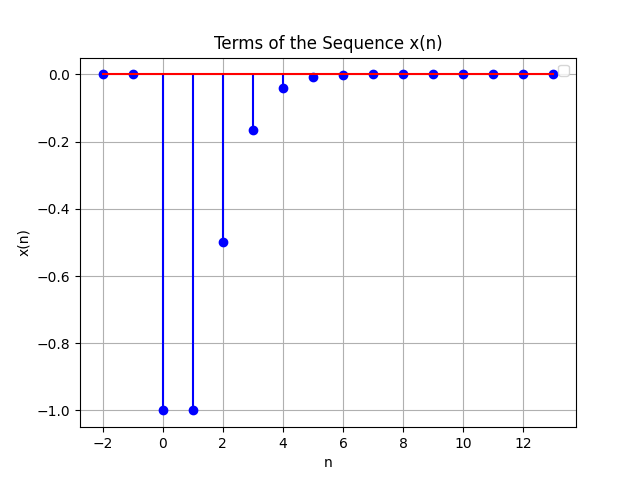
\includegraphics[width=1\columnwidth]{ncert-maths/11/9/1/12/figs/plot.png}
   \caption{Plot of x(n) vs n}
   \label{fig: 9.1.12.1}
\end{figure}

\begin{align}
    X \brak{z} & = \sum_{n=-\infty}^{\infty} x \brak{n}   z^{-n} \\
    \notag \text{using \eqref{x(n)}, } \\
    & = \sum_{n=-\infty}^{\infty} \frac{-1}{n!}  u \brak{n}   z^{-n} \\
    & = \sum_{n=0}^{\infty} \frac{-1}{n!}   z^{-n} \\
    & = - e^{z^{-1}} &  \cbrak{z\in\mathbb{C} : z \neq 0} 
\end{align}

\begin{table}[h]
    \centering
      \begin{tabular}{|c|c|c|}
    \hline
    	\textbf{Symbol} & \textbf{Value} & \textbf{Description} \\
    \hline
	  $x(n)$ & $\frac{-1}{n!}$ & general term of the series \\
    \hline
	  $X(z)$ & $- e^{z^{-1}}$ &Z-transform of x(n) \\
    \hline 
	  $u(n)$ & &unit step function \\
    \hline
  \end{tabular}

    \caption{Parameters}
    \label{tab: 9.1.12.1}
\end{table}


%\end{document}

\pagebreak


\item Subba Rao started work in 1995 at an annual salary of Rs. 5000 and received an increment of Rs. 200 each year. In which year did his income reach Rs. 7000?

\solution

\iffalse
\let\negmedspace\undefined
\let\negthickspace\undefined
\documentclass[journal,12pt,twocolumn]{IEEEtran}
\usepackage{cite}
\usepackage{amsmath,amssymb,amsfonts,amsthm}
\usepackage{algorithmic}
\usepackage{graphicx}
\usepackage{textcomp}
\usepackage{xcolor}
\usepackage{txfonts}
\usepackage{listings}
\usepackage{enumitem}
\usepackage{mathtools}
\usepackage{gensymb}
\usepackage{comment}
\usepackage[breaklinks=true]{hyperref}
\usepackage{tkz-euclide}
\usepackage{listings}
\usepackage{gvv}
\def\inputGnumericTable{}
\usepackage[latin1]{inputenc}
\usepackage{color}
\usepackage{array}
\usepackage{longtable}
\usepackage{calc}
\usepackage{multirow}
\usepackage{hhline}
\usepackage{ifthen}
\usepackage{lscape}

\newtheorem{theorem}{Theorem}[section]
\newtheorem{problem}{Problem}
\newtheorem{proposition}{Proposition}[section]
\newtheorem{lemma}{Lemma}[section]
\newtheorem{corollary}[theorem]{Corollary}
\newtheorem{example}{Example}[section]
\newtheorem{definition}[problem]{Definition}
\newcommand{\BEQA}{\begin{eqnarray}}
\newcommand{\EEQA}{\end{eqnarray}}
\newcommand{\define}{\stackrel{\triangle}{=}}
\theoremstyle{remark}
\newtheorem{rem}{Remark}
\begin{document}

\bibliographystyle{IEEEtran}
\vspace{3cm}

\title{NCERT Discrete - 10.5.2.19}
\author{EE23BTECH11007 - Aneesh Kadiyala$^{*}$% <-this % stops a space
}
\maketitle
\newpage
\bigskip

\renewcommand{\thefigure}{\theenumi}
\renewcommand{\thetable}{\theenumi}
\vspace{3cm}
\textbf{Question 10.5.2.19:} Subba Rao started work in 1995 at an annual salary of Rs. 5000 and received an increment of Rs. 200 each year. In which year did his income reach Rs. 7000?

\solution
\fi
\begin{table}[h!]
    \centering
    \begin{tabular}{ | c | c | c | }
        \hline
        Parameter & Value & Description \\
        \hline
        $x(0)$ & 5000 & Initial Income \\
        \hline
        $d$ & 200 & Annual Increment (Common Difference) \\
        \hline
        $x(n)$ & $(x(0) + nd)u(n)$ & $n^{th}$ term of the AP \\
        \hline
    \end{tabular}
    \caption{Input Parameters}
    \label{tab:math_10_5_2_19}
\end{table}
From the values given in \tabref{tab:math_10_5_2_19}:
\begin{align}
7000 &= 5000 + 200n \\
\implies 2000 &= 200n \\
\therefore n &= 10
\end{align}
\begin{figure}[h!]
    \centering
    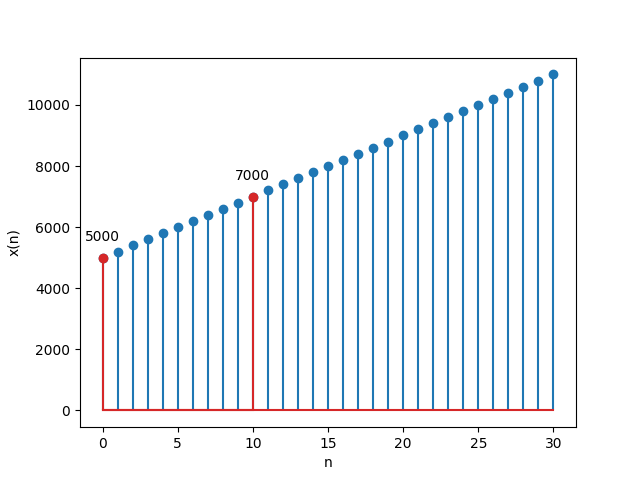
\includegraphics[width=\columnwidth]{ncert-maths/10/5/2/19/figs/10_5_2_19.png}
    \caption{Plot of $x(n)$ vs $n$. See \tabref{tab:math_10_5_2_19} for details.}
    \label{fig:math_10_5_2_19}
\end{figure}
Let Z-transform of $x(n)$ be $X(z)$.
\begin{align}
X(z) &= \frac{x(0)}{1 - z^{-1}} + \frac{dz^{-1}}{(1 - z^{-1})^2} \quad |z| > 1
\end{align}
Using the values from \tabref{tab:math_10_5_2_19}:
\begin{align}
X(z) &= \frac{5000}{1 - z^{-1}} + \frac{200z^{-1}}{(1 - z^{-1})^2} \quad |z| > 1
\end{align}
%\end{document}


\item Consider the sequence whose $n^\text{th}$ term is given by \(2^n\). Find the first 6 terms of this sequence.

\solution

%\iffalse
\let\negmedspace\undefined
\let\negthickspace\undefined
\documentclass[journal,12pt,onecolumn]{IEEEtran}
\usepackage{cite}
\usepackage{amsmath,amssymb,amsfonts,amsthm}
%\usepackage{algorithmic}
\usepackage{graphicx}
\usepackage{textcomp}
\usepackage{array}
\usepackage{xcolor}
\usepackage{txfonts}
\usepackage{listings}
\usepackage{enumitem}
\usepackage{mathtools}
\usepackage{gensymb}
\usepackage[breaklinks=true]{hyperref}
\usepackage{tkz-euclide} % loads  TikZ and tkz-base
\usepackage{listings}
\usepackage{float}



\newtheorem{theorem}{Theorem}[section]
\newtheorem{problem}{Problem}
\newtheorem{proposition}{Proposition}[section]
\newtheorem{lemma}{Lemma}[section]
\newtheorem{corollary}[theorem]{Corollary}
\newtheorem{example}{Example}[section]
\newtheorem{definition}[problem]{Definition}
%\newtheorem{thm}{Theorem}[section] 
%\newtheorem{defn}[thm]{Definition}
%\newtheorem{algorithm}{Algorithm}[section]
%\newtheorem{cor}{Corollary}
\newcommand{\BEQA}{\begin{eqnarray}}
\newcommand{\EEQA}{\end{eqnarray}}
\newcommand{\define}{\stackrel{\triangle}{=}}
\theoremstyle{remark}
\newtheorem{rem}{Remark}
%\bibliographystyle{ieeetr}
\begin{document}
%
\providecommand{\pr}[1]{\ensuremath{\Pr\left(#1\right)}}
\providecommand{\prt}[2]{\ensuremath{p_{#1}^{\left(#2\right)} }}        % own macro for this question
\providecommand{\qfunc}[1]{\ensuremath{Q\left(#1\right)}}
\providecommand{\sbrak}[1]{\ensuremath{{}\left[#1\right]}}
\providecommand{\lsbrak}[1]{\ensuremath{{}\left[#1\right.}}
\providecommand{\rsbrak}[1]{\ensuremath{{}\left.#1\right]}}
\providecommand{\brak}[1]{\ensuremath{\left(#1\right)}}
\providecommand{\lbrak}[1]{\ensuremath{\left(#1\right.}}
\providecommand{\rbrak}[1]{\ensuremath{\left.#1\right)}}
\providecommand{\cbrak}[1]{\ensuremath{\left\{#1\right\}}}
\providecommand{\lcbrak}[1]{\ensuremath{\left\{#1\right.}}
\providecommand{\rcbrak}[1]{\ensuremath{\left.#1\right\}}}
\newcommand{\sgn}{\mathop{\mathrm{sgn}}}
\providecommand{\abs}[1]{\left\vert#1\right\vert}
\providecommand{\res}[1]{\Res\displaylimits_{#1}} 
\providecommand{\norm}[1]{\left\lVert#1\right\rVert}
%\providecommand{\norm}[1]{\lVert#1\rVert}
\providecommand{\mtx}[1]{\mathbf{#1}}
\providecommand{\mean}[1]{E\left[ #1 \right]}
\providecommand{\cond}[2]{#1\middle|#2}
\providecommand{\fourier}{\overset{\mathcal{F}}{ \rightleftharpoons}}
\newenvironment{amatrix}[1]{%
  \left(\begin{array}{@{}*{#1}{c}|c@{}}
}{%
  \end{array}\right)
}
%\providecommand{\hilbert}{\overset{\mathcal{H}}{ \rightleftharpoons}}
%\providecommand{\system}{\overset{\mathcal{H}}{ \longleftrightarrow}}
	%\newcommand{\solution}[2]{\textbf{Solution:}{#1}}
\newcommand{\solution}{\noindent \textbf{Solution: }}
\newcommand{\cosec}{\,\text{cosec}\,}
\providecommand{\dec}[2]{\ensuremath{\overset{#1}{\underset{#2}{\gtrless}}}}
\newcommand{\myvec}[1]{\ensuremath{\begin{pmatrix}#1\end{pmatrix}}}
\newcommand{\mydet}[1]{\ensuremath{\begin{vmatrix}#1\end{vmatrix}}}
\newcommand{\myaugvec}[2]{\ensuremath{\begin{amatrix}{#1}#2\end{amatrix}}}
\providecommand{\rank}{\text{rank}}
\providecommand{\pr}[1]{\ensuremath{\Pr\left(#1\right)}}
\providecommand{\qfunc}[1]{\ensuremath{Q\left(#1\right)}}
	\newcommand*{\permcomb}[4][0mu]{{{}^{#3}\mkern#1#2_{#4}}}
\newcommand*{\perm}[1][-3mu]{\permcomb[#1]{P}}
\newcommand*{\comb}[1][-1mu]{\permcomb[#1]{C}}
\providecommand{\qfunc}[1]{\ensuremath{Q\left(#1\right)}}
\providecommand{\gauss}[2]{\mathcal{N}\ensuremath{\left(#1,#2\right)}}
\providecommand{\diff}[2]{\ensuremath{\frac{d{#1}}{d{#2}}}}
\providecommand{\myceil}[1]{\left \lceil #1 \right \rceil }
\newcommand\figref{Fig.~\ref}
\newcommand\tabref{Table~\ref}
\newcommand{\sinc}{\,\text{sinc}\,}
\newcommand{\rect}{\,\text{rect}\,}
%%
%	%\newcommand{\solution}[2]{\textbf{Solution:}{#1}}
%\newcommand{\solution}{\noindent \textbf{Solution: }}
%\newcommand{\cosec}{\,\text{cosec}\,}
%\numberwithin{equation}{section}
%\numberwithin{equation}{subsection}
%\numberwithin{problem}{section}
%\numberwithin{definition}{section}
%\makeatletter
%\@addtoreset{figure}{problem}
%\makeatother

%\let\StandardTheFigure\thefigure
\let\vec\mathbf

\bibliographystyle{IEEEtran}





\bigskip

%\renewcommand{\thefigure}{\theenumi}
%\renewcommand{\thetable}{\theenumi}
%\renewcommand{\theequation}{\theenumi}

Q: Consider the sequence whose $n^\text{th}$ term is given by \(2^n\). Find the first 6 terms of this sequence.

\solution

\begin{table}[!ht]
    \centering
        \begin{table}[ht]
    \centering
    \begin{tabular}{|c|c|c|}
        \hline
        Parameter & Value & Description \\
        \hline
        $x(0)$ & 5 & First term of AP \\
        $d$ & 1.75 & Common difference of AP \\
        $x(n)$ & 20.75 & $n^{th}$ term of AP \\
        \hline
    \end{tabular}
    \vspace{2mm}
    \caption{Parameter List}
    \label{tab:simple.10.5.2.20}
\end{table}

    \caption{input parameters}
    \label{tab:11_9_1_3}
\end{table}
%\fi
\begin{align}
X(Z) &= \frac {1}{1 - 2  z^{-1} } \quad \abs{z}>\abs{2}
\end{align}

\begin{figure}[H]
    \centering
    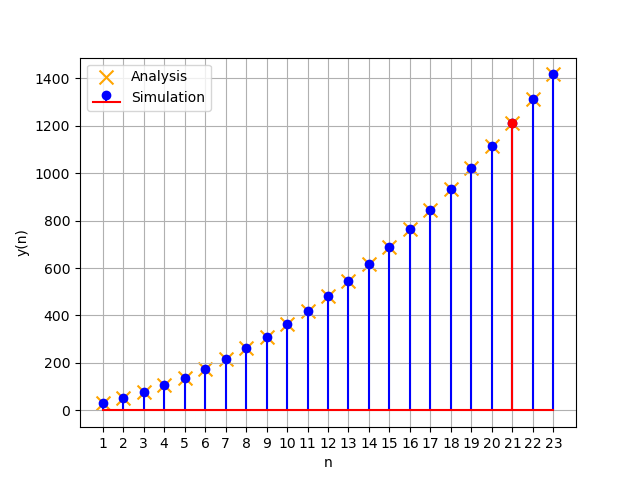
\includegraphics{figs/fig1.png}
    \caption{Six terms of given sequence}
    \label{fig:11_9_1_3 }
\end{figure}

\end{document}


\item If the sum of first 7 terms of an AP is 49 and that of 17 terms is 289, find the sum of first n terms.

\solution

\iffalse
\let\negmedspace\undefined
\let\negthickspace\undefined
\documentclass[journal,12pt,twocolumn]{IEEEtran}
\usepackage{cite}
\usepackage{amsmath,amssymb,amsfonts,amsthm}
\usepackage{algorithmic}
\usepackage{graphicx}
\usepackage{textcomp}
\usepackage{xcolor}
\usepackage{txfonts}
\usepackage{listings}
\usepackage{enumitem}
\usepackage{mathtools}
\usepackage{gensymb}
\usepackage{comment}
\usepackage[breaklinks=true]{hyperref}
\usepackage{tkz-euclide} 
\usepackage{listings}
\usepackage{gvv}                                        
\def\inputGnumericTable{}                                 
\usepackage[latin1]{inputenc}                                
\usepackage{color}                                            
\usepackage{array}                                            
\usepackage{longtable}                                       
\usepackage{calc}                                             
\usepackage{multirow}                                         
\usepackage{hhline}                                           
\usepackage{ifthen}                                           
\usepackage{lscape}
\newtheorem{theorem}{Theorem}[section]
\newtheorem{problem}{Problem}
\newtheorem{proposition}{Proposition}[section]
\newtheorem{lemma}{Lemma}[section]
\newtheorem{corollary}[theorem]{Corollary}
\newtheorem{example}{Example}[section]
\newtheorem{definition}[problem]{Definition}
\newcommand{\BEQA}{\begin{eqnarray}}
\newcommand{\EEQA}{\end{eqnarray}}
\newcommand{\define}{\stackrel{\triangle}{=}}
\theoremstyle{remark}
\newtheorem{rem}{Remark}
\begin{document}

\bibliographystyle{IEEEtran}
\vspace{3cm}

\title{10.5.3.9}
\author{EE23BTECH11063 - Vemula Siddhartha
}
\maketitle
\newpage
\bigskip

\renewcommand{\thefigure}{\theenumi}
\renewcommand{\thetable}{\theenumi}
\textbf{Question}:\\
If the sum of first 7 terms of an AP is 49 and that of 17 terms is 289, find the sum of
first n terms.
\\
\textbf{Solution: }
\fi
\begin{table}[h!]    
  \centering
  \begin{tabular}[12pt]{ |c| c|}
    \hline
    \textbf{Variable} & \textbf{Description}\\ 
    \hline
    $x\brak{0}$ & First term of the AP \\
    \hline 
    $d$ & Common difference of the AP\\
    \hline
    $y\brak{n}$ & Sum of $n+1$ terms of the AP\\
    \hline
    $x\brak{n}$ & General term\\
    \hline   
    \end{tabular}
  \caption{Variables Used}
  \label{tab10.5.3.9.1}
\end{table}
\begin{align}
y\brak{n}&=\frac{n+1}{2}\,\brak{2x\brak{0}+nd}\,u\brak{n}\label{eq10.5.3.9.1}\\
y\brak{6}&=49\\
y\brak{16}&=289
\end{align}
Then,
\begin{align}
x\brak{0}+3d&=7\label{eq10.5.3.9.2}\\
x\brak{0}+8d&=17 \label{eq10.5.3.9.3}
\end{align}
From  equations \ref{eq10.5.3.9.2} and \ref{eq10.5.3.9.3}, the augmented matrix is:
\begin{align}
 \myvec{
   1 & 3 & 7
   \\
   1 & 8 & 17
 }
 \xleftrightarrow[]{R_2 \leftarrow {R_2-R_1}}
 \myvec{
   1 & 3 & 7
   \\
   0 & 5 & 10
 }
 \\
 \xleftrightarrow[]{R_1 \leftarrow {R_1-\frac{3}{5}R_2}}
 \myvec{
   1 & 0 & 1
   \\
   0 & 5 & 10
 }
 \\
 \xleftrightarrow[]{R_2 \leftarrow \frac{R_2}{5}}
 \myvec{
   1 & 0 & 1
   \\
   0 & 1 & 2
 }
 \\
 \implies \myvec{
   x\brak{0}
   \\
   d
 }
 =
 \myvec{
   1
   \\
   2
 }
\end{align}
\begin{align}
    x\brak{n}&= \brak{1+2n}u\brak{n}\\
    X\brak{z}&=\frac{1}{1-z^{-1}}+\frac{2z^{-1}}{\brak{1-z^{-1}}^2}\;\;\cbrak{z\in\mathbb{C}: |z|>1}
\end{align}
\begin{align}
   y\brak{n}&=x\brak{n}*u\brak{n}\\
   Y\brak{z}&=X\brak{z}\,U\brak{z}\\
   \implies Y\brak{z}&=\brak{\frac{1}{1-z^{-1}}+\frac{2z^{-1}}{\brak{1-z^{-1}}^2}}\brak{\frac{1}{1-z^{-1}}}\\
   &=\frac{1}{\brak{1-z^{-1}}^2}+\frac{2z^{-1}}{\brak{1-z^{-1}}^3}\\
   \brak{n+1}u\brak{n}&\system{Z}\frac{1}{\brak{1-z^{-1}}^2}\cbrak{z\in\mathbb{C}: |z|>1}\\
   n\brak{\brak{n+1}u\brak{n}}&\system{Z}\frac{2z^{-1}}{\brak{1-z^{-1}}^3}\cbrak{z\in\mathbb{C}: |z|>1}
\end{align}
   From equations \eqref{eq:uzder-shift} and \eqref{eq:uzder-der}, taking the inverse Z Transform,
   \begin{align}
   y\brak{n}&=\brak{n+1}u\brak{n}+n\brak{\brak{n+1}u\brak{n}}\\
   \implies y\brak{n}&=\brak{n+1}^2\,u\brak{n}
\end{align}
\begin{figure}[h!]
   \centering
   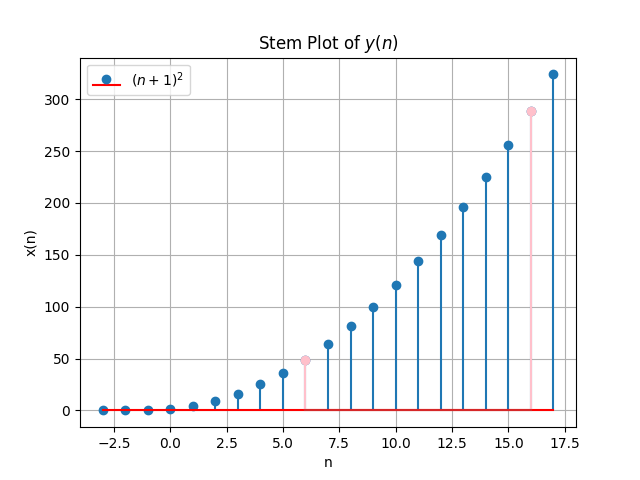
\includegraphics[width=1.1\linewidth]{ncert-maths/10/5/3/9/figs/Figure_1.png}
   \caption{Stem Plot of y\brak{n}}
   \label{stemplot}
\end{figure}  

\pagebreak

\item Write the first five terms of the sequence and obtain the corresponding series:\\
$a_1=a_2=2,$ $a_n=a_{n-1} -1,$ $n>2$\\
\solution
\iffalse
\let\negmedspace\undefined
\let\negthickspace\undefined
\documentclass[journal,12pt,twocolumn]{IEEEtran}
\usepackage{cite}
\usepackage{amsmath,amssymb,amsfonts,amsthm}
\usepackage{algorithmic}
\usepackage{graphicx}
\usepackage{textcomp}
\usepackage{xcolor}
\usepackage{txfonts}
\usepackage{listings}
\usepackage{enumitem}
\usepackage{mathtools}
\usepackage{float}
\usepackage{gensymb}
\usepackage{comment}
\usepackage[breaklinks=true]{hyperref}
\usepackage{tkz-euclide} 
\usepackage{listings}
\usepackage{gvv}                                        
\def\inputGnumericTable{}                                 
\usepackage[latin1]{inputenc}                                
\usepackage{color}                                            
\usepackage{array}                                            
\usepackage{longtable}                                       
\usepackage{calc}                                             
\usepackage{multirow}                                         
\usepackage{hhline}                                           
\usepackage{ifthen}                                           
\usepackage{lscape}
\usepackage{amsmath}
\newtheorem{theorem}{Theorem}[section]
\newtheorem{problem}{Problem}
\newtheorem{proposition}{Proposition}[section]
\newtheorem{lemma}{Lemma}[section]
\newtheorem{corollary}[theorem]{Corollary}
\newtheorem{example}{Example}[section]
\newtheorem{definition}[problem]{Definition}
\newcommand{\BEQA}{\begin{eqnarray}}
\newcommand{\EEQA}{\end{eqnarray}}
\newcommand{\define}{\stackrel{\triangle}{=}}
\theoremstyle{remark}
\newtheorem{rem}{Remark}
\begin{document}
\bibliographystyle{IEEEtran}
\title{NCERT 11.9.1.13Q}
\author{EE23BTECH11015 - DHANUSH V NAYAK$^{*}$% <-this % stops a space
}
\maketitle
\newpage
\bigskip
\renewcommand{\thefigure}{\arabic{figure}}
\renewcommand{\thetable}{\theenumi}
\textbf{Question:} Write the first five terms of each of the sequences in Exercises 11 to 13 and obtain the corresponding series:\\
$a_1=a_2=2,$\hspace{5pt} $a_n=a_{n-1} -1,$\hspace{5pt} $n>2$\\
\solution
\fi
\begin{table}[H]
    \centering
    \renewcommand\thetable{1}
    \setlength{\extrarowheight}{9pt}
    \resizebox{0.5\textwidth}{!}{
    \begin{tabular}{|c|c|c|}
    \hline
    \textbf{Parameter} & \textbf{Description} & \textbf{Value} \\ \hline
    $x\brak{0}$ & First term &2 \\ \hline
    $x\brak{1}$ & Second term &2 \\ \hline
    ROC & Region of convergence & $\left\{ z : \left|\sum_{n=-\infty}^{\infty} x(n)z^{-n}\right| < \infty \vphantom {\brak{{0.3pt}}}\right\}$ \\ \hline 
    $x(n)$ & General term & $x(n) = 
    \begin{cases}
        ? & ; n \geq 0 \\
        0 & ; n < 0 \\
    \end{cases}$ \\ \hline
    \end{tabular}}
    \caption{Parameter Table}
    \label{tab:11.9.1.13}
    \end{table}
\begin{align}
    x\brak{n} - x\brak{n-1} &= 2u\brak{n}-2u\brak{n-1}-u\brak{n-2}\label{eq:11.9.1.13.1}\\
X\brak{z}- z^{-1}X\brak{z} &= \frac{2}{\brak{1-z^{-1}}} - \frac{z^{-2}}{\brak{1-z^{-1}}}- \frac{2z^{-1}}{\brak{1-z^{-1}}}\\
    X\brak{z} &= \frac{2-2z^{-1}-z^{-2}}{\brak{1-z^{-1}}^2}  ,   \abs{z} >1
\end{align}
Using partial fractions
\begin{align}
    X\brak{z} &= \frac{2z^{-1}}{\brak{1-z^{-1}}} - \frac{z^{-2}}{\brak{1-z^{-1}}^2} + 2\label{eq:11.9.1.13.5}
\end{align}
Taking inverse $Z$-transform by result of equation \eqref{eq:11.9.5.26.9} in equation \eqref{eq:11.9.1.13.5}:
\begin{align}
    x\brak{n} &= 2u\brak{n}+\brak{1-n}u\brak{n-1}\label{eq:11.9.1.13.6}
\end{align}
\begin{figure}[H]
    \centering
    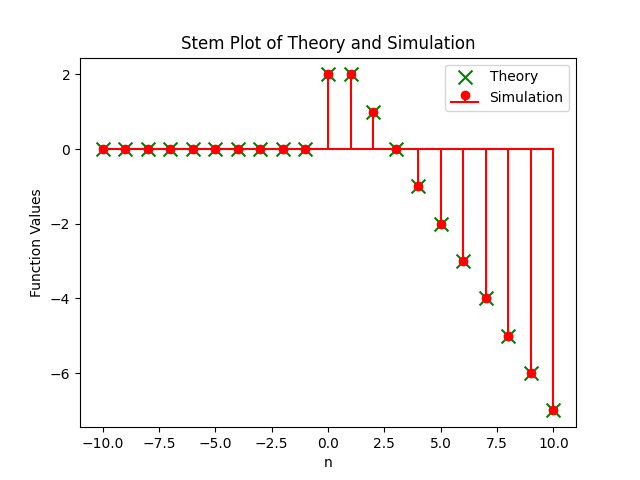
\includegraphics[width=1\columnwidth]{ncert-maths/11/9/1/13/figs/Theory_vs_Simulation.png}
    \caption{Comparison of Theory and Simulated Values}
    \label{fig:11.9.1.13.1}
\end{figure}
From the figure\figref{fig:11.9.1.13.1} we can see that the theoretical and simulated values overlap. 
%\end{document}

\pagebreak
\item Insert two numbers between 3 and 81 so that the resulting sequence is G.P.\\

\solution
\iffalse
\let\negmedspace\undefined
\let\negthickspace\undefined
\documentclass[journal,12pt,twocolumn]{IEEEtran}
\usepackage{cite}
\usepackage{amsmath,amssymb,amsfonts,amsthm}
\usepackage{algorithmic}
\usepackage{graphicx}
\usepackage{textcomp}
\usepackage{xcolor}
\usepackage{txfonts}
\usepackage{listings}
\usepackage{enumitem}
\usepackage{mathtools}
\usepackage{gensymb}
\usepackage{comment}
\usepackage[breaklinks=true]{hyperref}
\usepackage{tkz-euclide}
\usepackage{listings}
\usepackage{gvv}
\def\inputGnumericTable{}
\usepackage[latin1]{inputenc}
\usepackage{color}
\usepackage{array}
\usepackage{longtable}
\usepackage{calc}
\usepackage{multirow}
\usepackage{hhline}
\usepackage{ifthen}
\usepackage{lscape}

\newtheorem{theorem}{Theorem}[section]
\newtheorem{problem}{Problem}
\newtheorem{proposition}{Proposition}[section]
\newtheorem{lemma}{Lemma}[section]
\newtheorem{corollary}[theorem]{Corollary}
\newtheorem{example}{Example}[section]
\newtheorem{definition}[problem]{Definition}
\newcommand{\BEQA}{\begin{eqnarray}}
\newcommand{\EEQA}{\end{eqnarray}}
\newcommand{\define}{\stackrel{\triangle}{=}}
\theoremstyle{remark}
\newtheorem{rem}{Remark}
\begin{document}

\bibliographystyle{IEEEtran}
\vspace{3cm}

\title{NCERT Discrete 11.9.3 -26}
\author{EE23BTECH11057 - Shakunaveti Sai Sri Ram Varun$^{}$% &lt;-this % stops a space
}
\maketitle
\newpage
\bigskip
\vspace{2cm}
\textbf{Question: }
Insert two numbers between 3 and 81 so that the resulting sequence is G.P.\\
\textbf{Solution}:
\fi
\begin{table}[htbp] 
\centering
\begin{tabular}{|c|c|c|}
    \hline
    \textbf{Parameter} & \textbf{Description} & \textbf{Value} \\
    \hline
    $x\brak{0}$ & First term of G.P. & 3 \\
    \hline
    $x\brak{3}$ & Fourth term of G.P. & 81 \\
    \hline
    $r$ & common ratio of G.P. & r \\
    \hline
\end{tabular}



\caption{input values}
\label{tab: Table 11.9.3.26.15}
\end{table}
\begin{enumerate}
\item 
\begin{align}
x\brak{n}=x\brak{0}r^{n}
\end{align}
from the values in \tabref{tab: Table 11.9.3.26.15}
\begin{align}
%x(0)&=3\\
%x(3)&=81\\
\frac{x\brak{0}r^3}{x\brak{0}}&=27\\
r&=3
\end{align}
$ \therefore $ Required numbers are 9 and 27.
\item 
\begin{align}
x\brak{n} &= 3^{n+1}u\brak{n} \label{eq:11.9.3.26.1}\\
X\brak{z} &= \frac{3}{1-3z^{-1}} \quad |z|>3 \label{eq:11.9.3.26.2}
\end{align}
\begin{figure}[h!]
    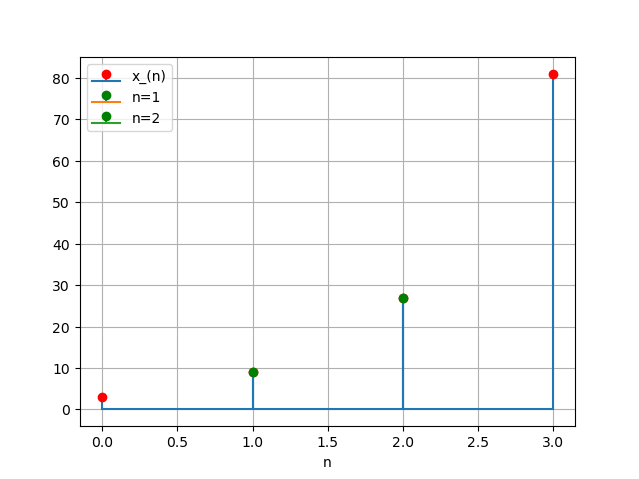
\includegraphics[width = \columnwidth]{ncert-maths/11/9/3/26/figs/Figure_1.png}
    \caption{Graph of $ x\brak{n}$ }
    \label{fig: 11.9.3.26.17}
\end{figure}
\end{enumerate}


\pagebreak

\item  What will Rs 500 amounts to in 10 years after its deposit in a bank which pays annual interest rate of 10$\%$ compounded annually?

\solution
    \let\negmedspace\undefined
\let\negthickspace\undefined
\documentclass[journal,12pt,twocolumn]{IEEEtran}
\usepackage{cite}
\usepackage{amsmath,amssymb,amsfonts,amsthm}
\usepackage{algorithmic}
\usepackage{graphicx}
\usepackage{textcomp}
\usepackage{xcolor}
\usepackage{txfonts}
\usepackage{listings}
\usepackage{enumitem}
\usepackage{mathtools}
\usepackage{gensymb}
\usepackage[breaklinks=true]{hyperref}
\usepackage{tkz-euclide} % loads  TikZ and tkz-base
\usepackage{listings}
\usepackage{gvv}


\newtheorem{theorem}{Theorem}[section]
\newtheorem{problem}{Problem}
\newtheorem{proposition}{Proposition}[section]
\newtheorem{lemma}{Lemma}[section]
\newtheorem{corollary}[theorem]{Corollary}
\newtheorem{example}{Example}[section]
\newtheorem{definition}[problem]{Definition}

\newcommand{\BEQA}{\begin{eqnarray}}
\newcommand{\EEQA}{\end{eqnarray}}
\newcommand{\define}{\stackrel{\triangle}{=}}
\theoremstyle{remark}
\newtheorem{rem}{Remark}

\graphicspath{./figs/}

%\bibliographystyle{ieeetr}
\begin{document}
%

\bibliographystyle{IEEEtran}


\vspace{3cm}

\title{
	%	\logo{
	Assignment-2

	\large{EE:1205 Signals and Systems}

	Indian Institute of Technology, Hyderabad
	%	}
}
\author{Kunal Thorawade

EE23BTECH11035
}	

\maketitle


\newpage

%\tableofcontents

\bigskip
 
 \renewcommand{\thefigure}{\theenumi}
 \renewcommand{\thetable}{\arabic{table}}
 %\renewcommand{\theequation}{\theenumi}

 \section{Question:}
 What will Rs 500 amounts to in 10 years after its deposit in a bank which pays annual interest rate of 10$\%$ compounded annually?

 \section{Solution}

 \begin{table}[ht]
    \centering
    \begin{tabular}{|c|c|c|}
        \hline
        Parameter & Value & Description \\
        \hline
        $x(0)$ & 5 & First term of AP \\
        $d$ & 1.75 & Common difference of AP \\
        $x(n)$ & 20.75 & $n^{th}$ term of AP \\
        \hline
    \end{tabular}
    \vspace{2mm}
    \caption{Parameter List}
    \label{tab:simple.10.5.2.20}
\end{table}


 The Z-transform of a sequence $x(n)$ is given by:

 \begin{align}
	     x(n) &= 500(1.1)^{n}u(n)
	       \\  X(Z) &= \frac{500}{1 - (1.1)z^{-1}} ; |z| > 1.1
 \end{align}

 \begin{figure}
	     \centering
	         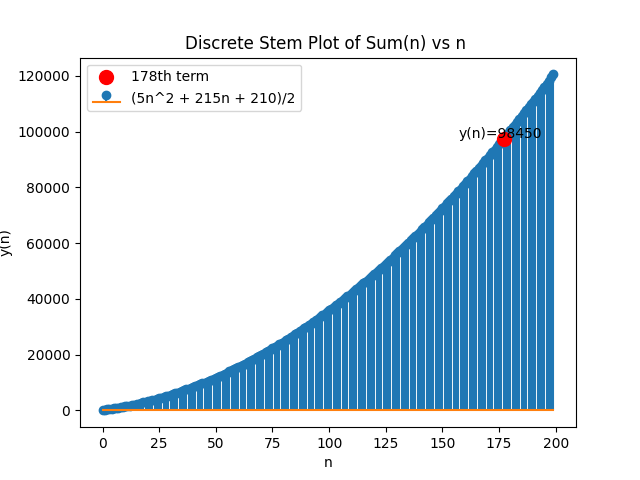
\includegraphics[width = 8cm]{figs/Fig1.png}
		     \caption{Plot of $x(n) = 500(1.1)^n$}
		         \label{fig:enter-label}
 \end{figure}
\end{document}

\pagebreak

\item Find the $20^{th}$ term from the last term of the AP: $3,8,13.....253$.

\solution
% \iffalse
\let\negmedspace\undefined
\let\negthickspace\undefined
\documentclass[journal,12pt,twocolumn]{IEEEtran}
\usepackage{cite}
\usepackage{amsmath,amssymb,amsfonts,amsthm}
\usepackage{algorithmic}
\usepackage{graphicx}
\usepackage{textcomp}
\usepackage{xcolor}
\usepackage{txfonts}
\usepackage{listings}
\usepackage{enumitem}
\usepackage{mathtools}
\usepackage{gensymb}
\usepackage{comment}
\usepackage[breaklinks=true]{hyperref}
\usepackage{tkz-euclide} 
\usepackage{listings}
\usepackage{gvv}                                        
\def\inputGnumericTable{}                                 
\usepackage[latin1]{inputenc}                                
\usepackage{color}                                            
\usepackage{array}                                            
\usepackage{longtable}                                       
\usepackage{calc}                                             
\usepackage{multirow}                                         
\usepackage{hhline}                                           
\usepackage{ifthen}                                           
\usepackage{lscape}
\usepackage{caption}
\newtheorem{theorem}{Theorem}[section]
\newtheorem{problem}{Problem}
\newtheorem{proposition}{Proposition}[section]
\newtheorem{lemma}{Lemma}[section]
\newtheorem{corollary}[theorem]{Corollary}
\newtheorem{example}{Example}[section]
\newtheorem{definition}[problem]{Definition}
\newcommand{\BEQA}{\begin{eqnarray}}
\newcommand{\EEQA}{\end{eqnarray}}
\newcommand{\define}{\stackrel{\triangle}{=}}
\theoremstyle{remark}
\newtheorem{rem}{Remark}
\begin{document}
\parindent 0px
\bibliographystyle{IEEEtran}
\vspace{3cm}

\title{NCERT 10.5.2 17Q}
\author{EE23BTECH11012 - Chavan Dinesh$^{*}$% <-this % stops a space
}
\maketitle
\newpage
\bigskip

\renewcommand{\thefigure}{\arabic{figure}}
\renewcommand{\thetable}{\arabic{table}}
\large\textbf{\textsl{Question:}}
Find the $20^{th}$ term from the last term of the AP: $3,8,13.....253$.

\solution

As the $20^{th}$ term is considered from last, 

\begin{table}[htbp]
    \centering
    \begin{table}[ht]
    \centering
    \begin{tabular}{|c|c|c|}
        \hline
        Parameter & Value & Description \\
        \hline
        $x(0)$ & 5 & First term of AP \\
        $d$ & 1.75 & Common difference of AP \\
        $x(n)$ & 20.75 & $n^{th}$ term of AP \\
        \hline
    \end{tabular}
    \vspace{2mm}
    \caption{Parameter List}
    \label{tab:simple.10.5.2.20}
\end{table}

    \caption{Input table}
    \label{tab:parameter_table.10.5.2.17}
\end{table}
% From \tabref{tab:parameter_table.10.5.2.17}:
% \begin{align}
%     x(n)&=x(0) + nd\\
%      x(19) &= 253 + (-5)19 \\
%         &= 158 
% \end{align}
% From \tabref{tab:parameter_table.10.5.2.17}:
% \begin{align}
% x(N-n)&=x(0) + (N-n)d\\
% x(N-19) &= 3 + (50 - 19)(5)\\
% &= 3 + 155\\
% &= 158
% \end{align}

From equation \eqref{eq:ztrans} and \eqref{eq:11.9.5.26.2}:
% \(Z\)-Transform of \(x(n)\):
\begin{align}
 X(z) =\frac{253}{1-z^{-1}}+ \frac{-5z^{-1}}{\brak{1-z^{-1}}^2};\cbrak{|z|>1}
\end{align}

\begin{figure}[ht]
    \centering
    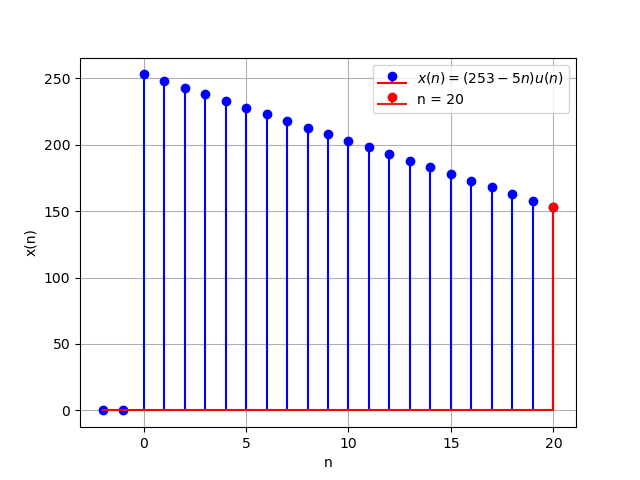
\includegraphics[width = \columnwidth]{figs/x(n)_vs_n.png}
    \caption{}
    \label{fig:graph1.10.5.2.17}
\end{figure}

\bibliographystyle{IEEEtran}
\end{document}


\pagebreak
\item Find the sum to $n$ terms of series , whose $n^{th}$ term is : $n(n+1)(n+4)$.

\solution
\iffalse
\documentclass[journal,12pt,twocolumn]{IEEEtran}
\usepackage{cite}
\usepackage{amsmath,amssymb,amsfonts,amsthm}
\usepackage{algorithmic}
\usepackage{graphicx}
\usepackage{textcomp}
\usepackage{xcolor}
\usepackage{txfonts}
\usepackage{listings}
\usepackage{enumitem}
\usepackage{mathtools}
\usepackage{gensymb}
\usepackage{comment}
\usepackage[breaklinks=true]{hyperref}
\usepackage{tkz-euclide}
\usepackage{listings}
\usepackage{gvv}
\def\inputGnumericTable{}
\usepackage[latin1]{inputenc}
\usepackage{color}
\usepackage{array}
\usepackage{longtable}
\usepackage{calc}
\usepackage{multirow}
\usepackage{hhline}
\usepackage{ifthen}
\usepackage{lscape}
\usepackage{caption}

\newtheorem{theorem}{Theorem}[section]
\newtheorem{problem}{Problem}
\newtheorem{proposition}{Proposition}[section]
\newtheorem{lemma}{Lemma}[section]
\newtheorem{corollary}[theorem]{Corollary}
\newtheorem{example}{Example}[section]
\newtheorem{definition}[problem]{Definition}
\newcommand{\BEQA}{\begin{eqnarray}}
\newcommand{\EEQA}{\end{eqnarray}}
\newcommand{\define}{\stackrel{\triangle}{=}}
\theoremstyle{remark}
\newtheorem{rem}{Remark}
\begin{document}

\bibliographystyle{IEEEtran}
\vspace{3cm}

\title{NCERT 11.9.4 8Q}
\author{EE23BTECH11010 - Venkatesh D Bandawar $^{*}$% <-this % stops a space
}
\maketitle
% \newpage
\bigskip

\renewcommand{\thefigure}{\theenumi}
\renewcommand{\thetable}{\theenumi}

\textbf{Question:} Find the sum to $n$ terms of series , whose $n^{th}$ term is : $n(n+1)(n+4)$.

\textbf{Solution}
\fi
\begin{table}[!h] 
\centering
\begin{tabular}{|c|c|c|}
\hline
\textbf{Parameter} & \textbf{Description} & \textbf{Value} \\
\hline
$x(n)$ & $n^{th}$ term of series & $n(n+1)(n+4)u(n)$\\
\hline
$y(n)$ & sum of n terms of series&\\
\hline
\end{tabular}

\caption{Given parameters}
\label{given parameters list.11.9.4.8}
\end{table}

\begin{align}
        n u(n) &\system{Z} \frac{z^{-1}}{\brak{1-z^{-1}}^2} \cbrak{\abs{z}>1} \label{eq:z transform of nu(n)} \\
        n^2 u(n) &\system{Z} \frac{z^{-1}\brak{1+z^{-1}}}{\brak{1-z^{-1}}^3} \cbrak{\abs{z}>1}\label{eq:z transform of n^2u(n)} \\
        n^3 u(n) &\system{Z} \frac{z^{-1}\brak{1+4z^{-1}+z^{-2}}}{\brak{1-z^{-1}}^4} \cbrak{\abs{z}>1}\label{eq:z transform of n^3u(n)} \\
        n^4 u(n) &\system{Z} \frac{z^{-1}\brak{1+11z^{-1}+11z^{-2}+z^{-3}}}{\brak{1-z^{-1}}^5} \cbrak{\abs{z}>1}\label{eq:z transform of n^4u(n)}
    \end{align}
From equation \eqref{eq:11.9.5.26.2} to \eqref{eq:11.9.5.26.4},\\
    \begin{multline}
        X(z) = \frac{z^{-1}\brak{1+4z^{-1}+z^{-2}}}{\brak{1-z^{-1}}^4} + \frac{5z^{-1}\brak{z^{-1}+1}}{\brak{1-z^{-1}}^3}\\ 
        + \frac{4z^{-1}}{\brak{1-z^{-1}}^2} \cbrak{\abs{z}>1}
    \end{multline}
    \begin{align}
         Y(z) &= X(z)U(z)\\
         &=\frac{z^{-1}\brak{1+4z^{-1}+z^{-2}}}{\brak{1-z^{-1}}^5} + \frac{5z^{-1}\brak{z^{-1}+1}}{\brak{1-z^{-1}}^4} + \frac{4z^{-1}}{\brak{1-z^{-1}}^3} 
    \end{align}
    \begin{multline}
        = \frac{1}{4}\sbrak{\frac{z^{-1}\brak{1+11z^{-1}+11z^{-2}+z^{-3}}}{\brak{1-z^{-1}}^5}} \\
        +\frac{13}{6}\sbrak{\frac{z^{-1}\brak{1+4z^{-1}+z^{-2}}}{\brak{1-z^{-1}}^4}} + \frac{19}{4}\sbrak{\frac{z^{-1}\brak{1+z^{-1}}}{\brak{1-z^{-1}}^3}}\\
        + \frac{17}{6}\sbrak{\frac{z^{-1}}{\brak{1-z^{-1}}^2}} \cbrak{\abs{z}>1}
    \end{multline}
    Taking reverse z transform, using equations \eqref{eq:z transform of nu(n)} to \eqref{eq:z transform of n^4u(n)}
    \begin{align}
        y(n) = \brak{\frac{n^4}{4} + \frac{13n^3}{6} + \frac{19n^2}{4} + \frac{17n}{6}} u\brak{n}
    \end{align}
    \begin{multline}
        = \brak{\frac{n^4}{4} + \frac{2n^3}{4} + \frac{10n^3}{6} + \frac{n^2}{4} + \frac{15n^2}{6} + \frac{4n^2}{2} + \frac{5n}{6} + \frac{4n}{2}} u\brak{n}
    \end{multline}
    \begin{multline}
        = \brak{\frac{n^4+2n^3+n^4}{4}}u\brak{n} +\brak{\frac{10n^3+15n^2+5n}{6}}u\brak{n}\\
        +\brak{\frac{4n^2+4n}{2}}u\brak{n}
    \end{multline}
    \begin{multline}
        = \brak{\frac{n^2\brak{n+1}^2}{4} + \frac{5n(n+1)(2n+1)}{6} 
        + \frac{4n(n+1)}{2}} u\brak{n}
    \end{multline}
    \begin{figure}[!h] 
    \centering
    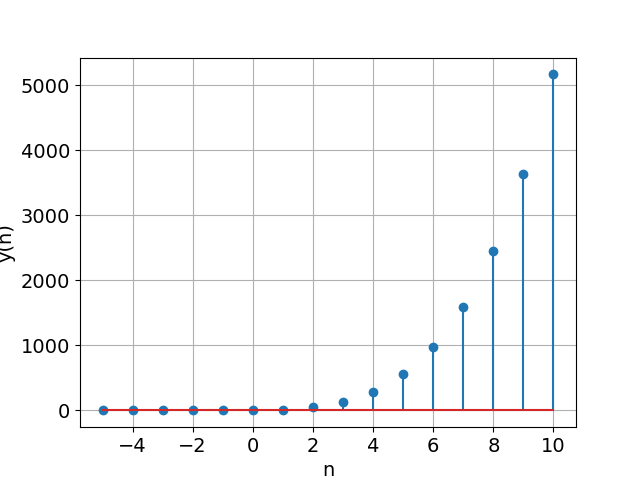
\includegraphics[width=\columnwidth]{ncert-maths/11/9/4/8/figs/sumplot.png}
    \caption{Sum of n terms of series}
    \label{fig:Graph1_math.11.9.4.8}
    \end{figure}


\pagebreak

\item Find the indicated terms in the sequence whose nth terms is $a(n)$ = $4n-3$. Find $a(17)$ and $a(24)$.
    
\solution 
\let\negmedspace\undefined
\let\negthickspace\undefined
\documentclass[journal,12pt,twocolumn]{IEEEtran}

\usepackage{cite}
\usepackage{amsmath,amssymb,amsfonts,amsthm}
\usepackage{algorithmic}
\usepackage{graphicx}
\usepackage{textcomp}
\usepackage{xcolor}
\usepackage{txfonts}
\usepackage{listings}
\usepackage{enumitem}
\usepackage{mathtools}
\usepackage{gensymb}
\usepackage[breaklinks=true]{hyperref}
\usepackage{tkz-euclide} % loads  TikZ and tkz-base
\usepackage{listings}
\usepackage{circuitikz}
\usepackage{graphicx}

%\newcounter{MYtempeqncnt}
\DeclareMathOperator*{\Res}{Res}
%\renewcommand{\baselinestretch}{2}
\renewcommand\thesection{\arabic{section}}
\renewcommand\thesubsection{\thesection.\arabic{subsection}}
\renewcommand\thesubsubsection{\thesubsection.\arabic{subsubsection}}

\renewcommand\thesectiondis{\arabic{section}}
\renewcommand\thesubsectiondis{\thesectiondis.\arabic{subsection}}
\renewcommand\thesubsubsectiondis{\thesubsectiondis.\arabic{subsubsection}}

% correct bad hyphenation here
\hyphenation{op-tical net-works semi-conduc-tor}
\def\inputGnumericTable{}                                 %%

\lstset{
	frame=single,
	breaklines=true,
	columns=fullflexible
}



\newtheorem{theorem}{Theorem}[section]
\newtheorem{problem}{Problem}
\newtheorem{proposition}{Proposition}[section]
\newtheorem{lemma}{Lemma}[section]
\newtheorem{corollary}[theorem]{Corollary}
\newtheorem{example}{Example}[section]
\newtheorem{definition}[problem]{Definition}
\newcommand{\BEQA}{\begin{eqnarray}}
	\newcommand{\EEQA}{\end{eqnarray}}
\newcommand{\define}{\stackrel{\triangle}{=}}
\newcommand\figref{Fig.~\ref}
\newcommand\tabref{Table~\ref}
\bibliographystyle{IEEEtran}
%\bibliographystyle{ieeetr}


\providecommand{\mbf}{\mathbf}
\providecommand{\pr}[1]{\ensuremath{\Pr\left(#1\right)}}
\providecommand{\qfunc}[1]{\ensuremath{Q\left(#1\right)}}
\providecommand{\sbrak}[1]{\ensuremath{{}\left[#1\right]}}
\providecommand{\lsbrak}[1]{\ensuremath{{}\left[#1\right.}}
\providecommand{\rsbrak}[1]{\ensuremath{{}\left.#1\right]}}
\providecommand{\brak}[1]{\ensuremath{\left(#1\right)}}
\providecommand{\lbrak}[1]{\ensuremath{\left(#1\right.}}
\providecommand{\rbrak}[1]{\ensuremath{\left.#1\right)}}
\providecommand{\cbrak}[1]{\ensuremath{\left\{#1\right\}}}
\providecommand{\lcbrak}[1]{\ensuremath{\left\{#1\right.}}
\providecommand{\rcbrak}[1]{\ensuremath{\left.#1\right\}}}
\theoremstyle{remark}
\newtheorem{rem}{Remark}
\newcommand{\sgn}{\mathop{\mathrm{sgn}}}
\providecommand{\abs}[1]{\left\vert#1\right\vert}
\providecommand{\res}[1]{\Res\displaylimits_{#1}}
\providecommand{\norm}[1]{\left\lVert#1\right\rVert}
%\providecommand{\norm}[1]{\lVert#1\rVert}
\providecommand{\mtx}[1]{\mathbf{#1}}
\providecommand{\mean}[1]{E\left[ #1 \right]}
\providecommand{\fourier}{\overset{\mathcal{F}}{ \rightleftharpoons}}
%\providecommand{\hilbert}{\overset{\mathcal{H}}{ \rightleftharpoons}}
\providecommand{\system}{\overset{\mathcal{H}}{ \longleftrightarrow}}
%\newcommand{\solution}[2]{\textbf{Solution:}{#1}}
\newcommand{\solution}{\noindent \textbf{Solution: }}
\newcommand{\cosec}{\,\text{cosec}\,}
\providecommand{\dec}[2]{\ensuremath{\overset{#1}{\underset{#2}{\gtrless}}}}
\newcommand{\myvec}[1]{\ensuremath{\begin{pmatrix}#1\end{pmatrix}}}
\newcommand{\mydet}[1]{\ensuremath{\begin{vmatrix}#1\end{vmatrix}}}
\renewcommand{\abstractname}{Question}

\let\vec\mathbf

	
	\vspace{3cm}
	
	


\newcommand{\permcomb}[4][0mu]{{{}^{#3}\mkern#1#2_{#4}}}
\newcommand{\comb}[1][-1mu]{\permcomb[#1]{C}}

%\IEEEpeerreviewmaketitle

\newcommand \tab [1][1cm]{\hspace*{#1}}
%\newcommand{\Var}{$\sigma ^2$}
\usepackage{amssymb}
\usepackage{amsmath}
\title{
	
\title{NCERT Discrete 11.9.1 Q7}
\author{EE23BTECH11061 - SWATHI DEEPIKA$^{*}$% <-this % stops a space
}


}
\begin{document}

\maketitle

\textbf{Question:} 
Find the indicated terms in the sequence whose nth terms is $a(n)$ = $4n-3$. Find $a(17)$ and $a(24)$.
    
\solution
In the question, following information is provided:
 
 \begin{table}[h]
 	\centering
 	\resizebox{6 cm}{!}{
 		\begin{table}[ht]
    \centering
    \begin{tabular}{|c|c|c|}
        \hline
        Parameter & Value & Description \\
        \hline
        $x(0)$ & 5 & First term of AP \\
        $d$ & 1.75 & Common difference of AP \\
        $x(n)$ & 20.75 & $n^{th}$ term of AP \\
        \hline
    \end{tabular}
    \vspace{2mm}
    \caption{Parameter List}
    \label{tab:simple.10.5.2.20}
\end{table}

 	}
 	\vspace{6 pt}
 	\caption{Parameters}
 	\label{tab:sw_tabel} 
 \end{table}

\begin{align}
x(n) = (4n+1)(u(n))
\end{align}

\begin{align}
 x(16) = 4 \times 16 + 1 = 65
\end{align}

\begin{align}
x(23) = 4 \times 23 + 1 = 93
\end{align}

Using Z-Transform,
\begin{align}
X(z) = 4\frac{z^{-1}}{(1-z^{-1})^2} + \frac{1}{1-z^{-1}}
 \quad |z| > 1
\end{align}

\begin{figure}[!h]
    \centering
    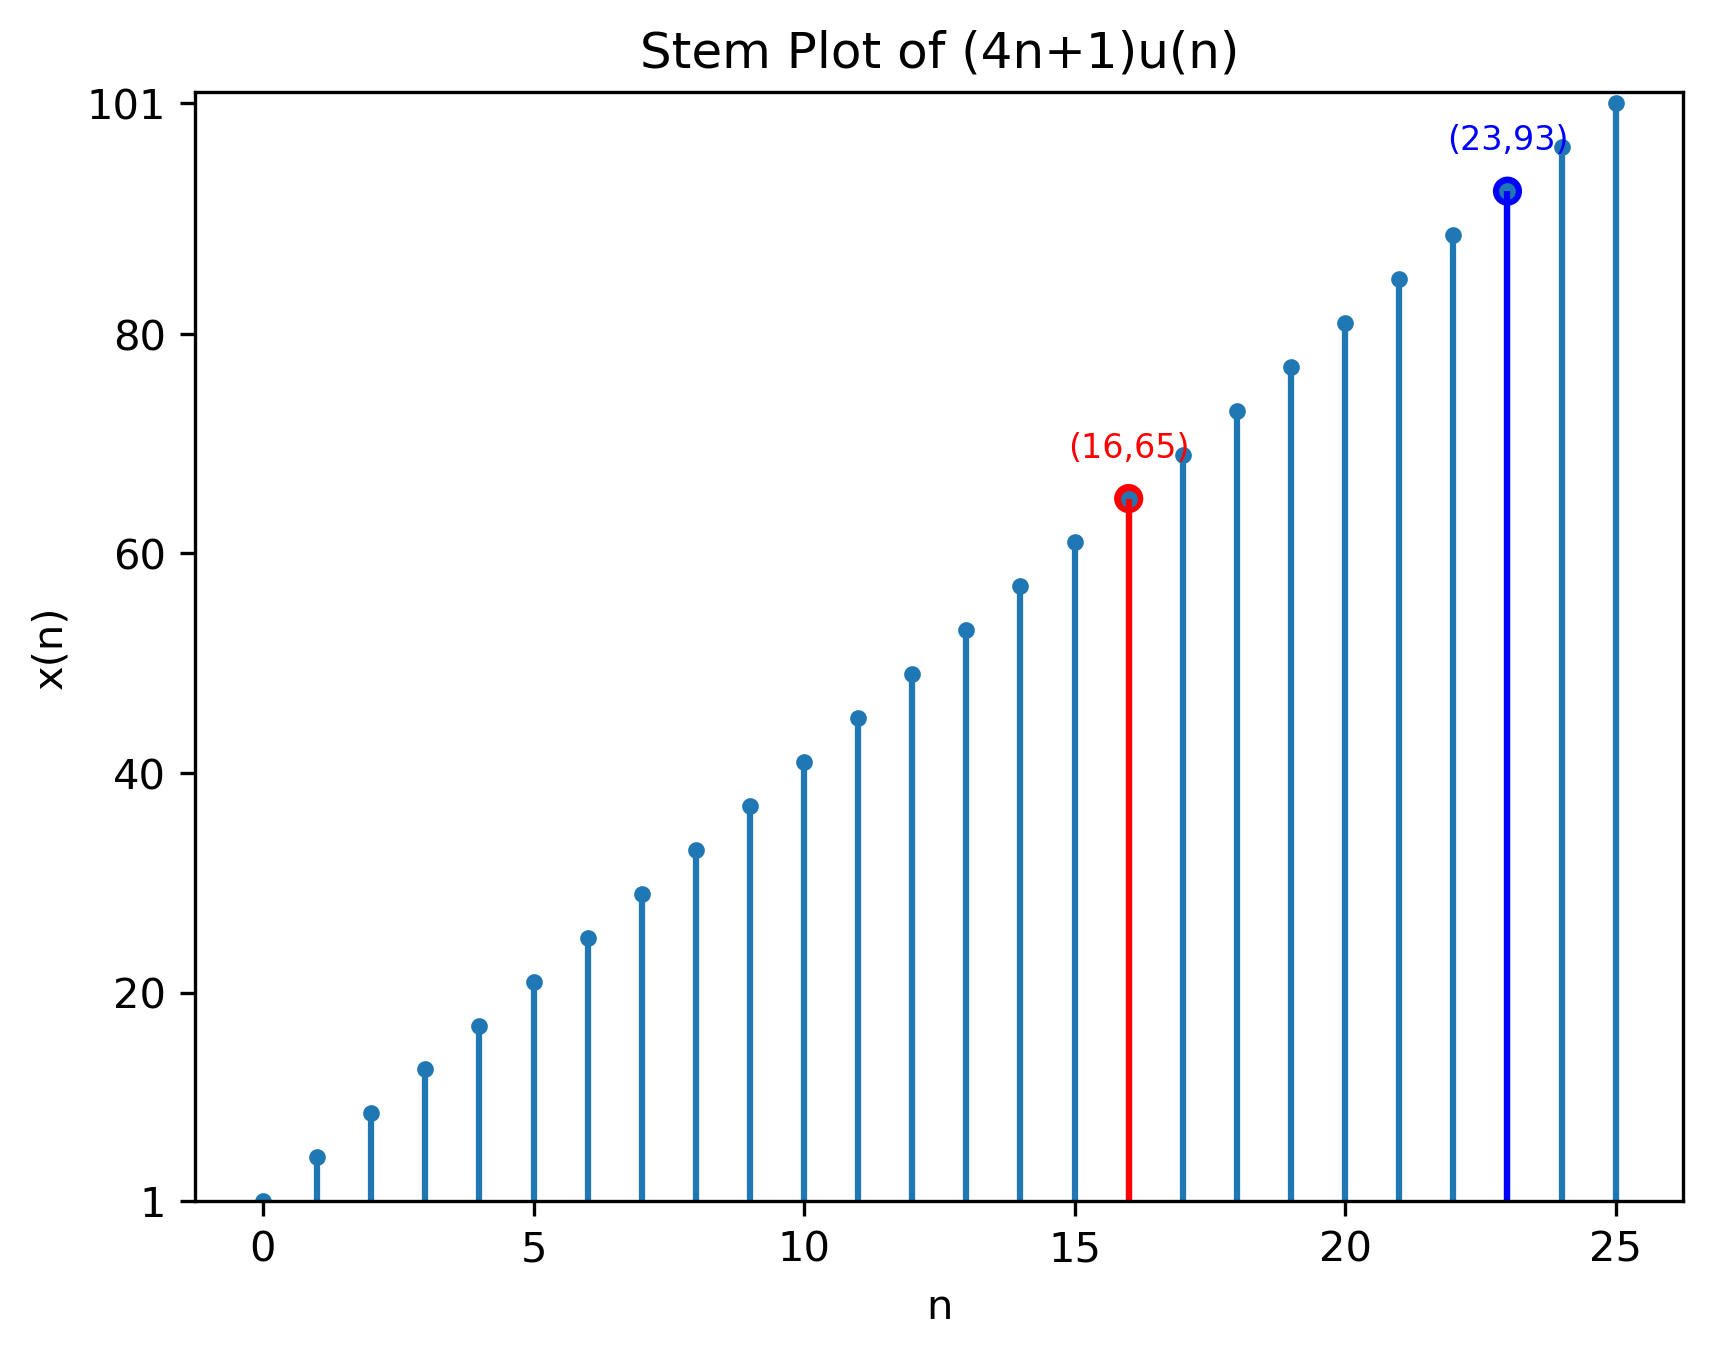
\includegraphics[width = \columnwidth]{figs/a_plot.png}
    \caption{$x(n)$ vs $n$}
    \label{fig:sw_plot}
\end{figure}



\end{document}




\pagebreak

\item The difference between any two cosecutive interior angles of a polygon is $5^\circ$.If the smallest angle is $120^\circ$,find the number of sides of polygon. \\
\solution
\iffalse
\let\negmedspace\undefined
\let\negthickspace\undefined
\documentclass[journal,12pt,twocolumn]{IEEEtran}
\usepackage{cite}
\usepackage{amsmath,amssymb,amsfonts,amsthm}
%\usepackage{algorithmic}
\usepackage{graphicx}
\usepackage{textcomp}
\usepackage{xcolor}
\usepackage{txfonts}
\usepackage{listings}
\usepackage{enumitem}
\usepackage{mathtools}
\usepackage{gensymb}
\usepackage{comment}
\usepackage[breaklinks=true]{hyperref}
\usepackage{tkz-euclide} % loads  TikZ and tkz-base
\usepackage{listings}
\usepackage[latin1]{inputenc}                                
\usepackage{color}                                            
\usepackage{array}                                            
\usepackage{longtable}                                       
\usepackage{calc}                                             
\usepackage{multirow}                                         
\usepackage{hhline}                                           
\usepackage{ifthen}                                           
\usepackage{lscape}
\usepackage{caption}
\usepackage{gvv}

\newtheorem{theorem}{Theorem}[section]
\newtheorem{problem}{Problem}
\newtheorem{proposition}{Proposition}[section]
\newtheorem{lemma}{Lemma}[section]
\newtheorem{corollary}[theorem]{Corollary}
\newtheorem{example}{Example}[section]
\newtheorem{definition}[problem]{Definition}
%\newtheorem{thm}{Theorem}[section] 
%\newtheorem{defn}[thm]{Definition}
%\newtheorem{algorithm}{Algorithm}[section]
%\newtheorem{cor}{Corollary}
\newcommand{\BEQA}{\begin{eqnarray}}
\newcommand{\system}[1]{\stackrel{#1}{\rightarrow}}
\newcommand{\EEQA}{\end{eqnarray}}
\newcommand{\define}{\stackrel{\triangle}{=}}
\theoremstyle{remark}
\newtheorem{rem}{Remark}
%\bibliographystyle{ieeetr}

\begin{document}
\providecommand{\pr}[1]{\ensuremath{\Pr\left(#1\right)}}
\providecommand{\prt}[2]{\ensuremath{p_{#1}^{\left(#2\right)} }}        % own macro for this question
\providecommand{\qfunc}[1]{\ensuremath{Q\left(#1\right)}}
\providecommand{\sbrak}[1]{\ensuremath{{}\left[#1\right]}}
\providecommand{\lsbrak}[1]{\ensuremath{{}\left[#1\right.}}
\providecommand{\rsbrak}[1]{\ensuremath{{}\left.#1\right]}}
\providecommand{\brak}[1]{\ensuremath{\left(#1\right)}}
\providecommand{\lbrak}[1]{\ensuremath{\left(#1\right.}}
\providecommand{\rbrak}[1]{\ensuremath{\left.#1\right)}}
\providecommand{\cbrak}[1]{\ensuremath{\left\{#1\right\}}}
\providecommand{\lcbrak}[1]{\ensuremath{\left\{#1\right.}}
\providecommand{\rcbrak}[1]{\ensuremath{\left.#1\right\}}}
\newcommand{\sgn}{\mathop{\mathrm{sgn}}}
\providecommand{\abs}[1]{\left\vert#1\right\vert}
\providecommand{\res}[1]{\Res\displaylimits_{#1}} 
\providecommand{\norm}[1]{\left\lVert#1\right\rVert}
%\providecommand{\norm}[1]{\lVert#1\rVert}
\providecommand{\mtx}[1]{\mathbf{#1}}
\providecommand{\mean}[1]{E\left[ #1 \right]}
\providecommand{\cond}[2]{#1\middle|#2}
\providecommand{\fourier}{\overset{\mathcal{F}}{ \rightleftharpoons}}
\newenvironment{amatrix}[1]{%
  \left(\begin{array}{@{}*{#1}{c}|c@{}}
}{%
  \end{array}\right)
}
%\providecommand{\hilbert}{\overset{\mathcal{H}}{ \rightleftharpoons}}
%\providecommand{\system}{\overset{\mathcal{H}}{ \longleftrightarrow}}
        %\newcommand{\solution}[2]{\textbf{Solution:}{#1}}
\newcommand{\solution}{\noindent \textbf{Solution: }}
\newcommand{\cosec}{\,\text{cosec}\,}
\providecommand{\dec}[2]{\ensuremath{\overset{#1}{\underset{#2}{\gtrless}}}}
\newcommand{\myvec}[1]{\ensuremath{\begin{pmatrix}#1\end{pmatrix}}}
\newcommand{\mydet}[1]{\ensuremath{\begin{vmatrix}#1\end{vmatrix}}}
\newcommand{\myaugvec}[2]{\ensuremath{\begin{amatrix}{#1}#2\end{amatrix}}}
\providecommand{\rank}{\text{rank}}
\providecommand{\pr}[1]{\ensuremath{\Pr\left(#1\right)}}
\providecommand{\qfunc}[1]{\ensuremath{Q\left(#1\right)}}
        \newcommand*{\permcomb}[4][0mu]{{{}^{#3}\mkern#1#2_{#4}}}
\newcommand*{\perm}[1][-3mu]{\permcomb[#1]{P}}
\newcommand*{\comb}[1][-1mu]{\permcomb[#1]{C}}
\providecommand{\qfunc}[1]{\ensuremath{Q\left(#1\right)}}
\providecommand{\gauss}[2]{\mathcal{N}\ensuremath{\left(#1,#2\right)}}
\providecommand{\diff}[2]{\ensuremath{\frac{d{#1}}{d{#2}}}}
\providecommand{\myceil}[1]{\left \lceil #1 \right \rceil }
\newcommand\figref{Fig.~\ref}
\newcommand\tabref{Table~\ref}
\newcommand{\sinc}{\,\text{sinc}\,}
\newcommand{\rect}{\,\text{rect}\,}
%%
%       %\newcommand{\solution}[2]{\textbf{Solution:}{#1}}
%\newcommand{\solution}{\noindent \textbf{Solution: }}
%\newcommand{\cosec}{\,\text{cosec}\,}
%\numberwithin{equation}{section}
%\numberwithin{equation}{subsection}
%\numberwithin{problem}{section}
%\numberwithin{definition}{section}
%\makeatletter
%\@addtoreset{figure}{problem}
%\makeatother

%\let\StandardTheFigure\thefigure
\let\vec\mathbf

\bibliographystyle{IEEEtran}

\vspace{3cm}
\title{Assignment}
\author{EE23BTECH11008 - Meenakshi}
\maketitle
\newpage
\bigskip

\renewcommand{\thefigure}{\theenumi}
\renewcommand{\thetable}{\theenumi}
%\renewcommand{\theequation}{\theenumi}
Q:The difference between any two cosecutive interior angles of a polygon is $5^\circ$.If the smallest angle is $120^\circ$,find the number of sides of polygon. \\
\solution
\fi
\begin{table}[!ht]
    \centering
         \begin{tabular}{|c|c|c|} 
      \hline
\textbf{Variable}& \textbf{Description}& \textbf{Value}\\\hline
$x(0)$& first term of AP& 120  \\\hline
    d& common difference of AP & 5\\\hline
    $x(n)$ & general  term of AP&none\\\hline
\end{tabular}

    \caption{input parameters}
    \label{tab:11_9_2_1}
\end{table}

Sum of interior angles of a polygon with $n+1$ sides is given by
\begin{align}
    S &= (n-1)180
\end{align}
Sum of $n$ terms of AP is given by
\begin{align}
    y(n) &= x(n)*u(n)
\end{align}
where $x(n) = 120 + 5n$
\begin{equation}
    x(n)*u(n)=(n-1)180 \label{eq:11.9.2.4.eq}
\end{equation}
\begin{align}
    Y(z) &= X(z)U(z) \\
    &= \left(\frac{x(0)}{1-z^{-1}} + \frac{dz^{-1}}{(1-z^{-1})^2}\right) \frac{1}{1-z^{-1}} \quad |z|>1\\
    &=\frac{120}{(1-z^{-1})^2} + \frac{5z^{-1}}{(1-z^{-1})^3} \quad |z|>1
\end{align}
\begin{align}
	\brak{n+1}u\brak{n}&\system{ Z}\left(\frac{1}{\brak{1-z^{-1}}^2}\right)\quad |z|>1\label{eq:11.9.2.18.9} \\
	\frac{\brak{n}\brak{n-1}}{2}u\brak{n-1} &\system{Z}\left(\frac{z^{-1}}{\brak{1-z^{-1}}^3}\right) \quad |z|>1\label{eq:11.9.2.18.10}
\end{align}
applying inverse Z-transform for each term and solving we get,
\begin{align}
    y\brak{n} &= \frac{n+1}{2}\brak{240+5n}u(n)
\end{align}
now from ~\eqref{eq:11.9.2.4.eq} 
\begin{align}
y(n) &= (n-1)180 \\
\frac{n+1}{2}\brak{240+5n}u(n) &= (n-1)180
\end{align}
now replace $n$ by $n-1$: 
\begin{align}
    n(235+5n) &= (n-2)360\\
    5n^2-125n+720 &= 0
\end{align}
\begin{align}
   n &= 16,9
\end{align}

\begin{figure}[h]
\centering
 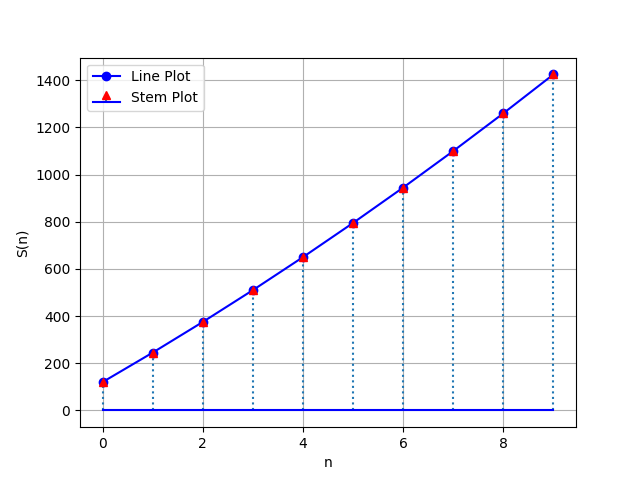
\includegraphics[width=\columnwidth]{ncert-maths/11/9/2/18/figs/python.1(1).png} 
  \captionsetup{justification=centering}
  \caption{Plot of the sum of n terms taken from Python}
  \label{fig:your_label}
\end{figure}

%\end{document}
   
   




\pagebreak
\item The $5$th,$8$th and $11$th terms of a GP are p,q and s respectively .show that $q^2=ps$ \\
\solution
\iffalse
\let\negmedspace\undefined
\let\negthickspace\undefined
\documentclass[journal,12pt,twocolumn]{IEEEtran}
\usepackage{cite}
\usepackage{amsmath,amssymb,amsfonts,amsthm}
\usepackage{algorithmic}
\usepackage{graphicx}
\usepackage{textcomp}
\usepackage{xcolor}
\usepackage{txfonts}
\usepackage{listings}
\usepackage{enumitem}
\usepackage{mathtools}
\usepackage{gensymb}
\usepackage{comment}
\usepackage[breaklinks=true]{hyperref}
\usepackage{tkz-euclide} 
\usepackage{listings}
\usepackage{gvv}                                        
\def\inputGnumericTable{}                                 
\usepackage[latin1]{inputenc}                                
\usepackage{color}                                            
\usepackage{array}                                            
\usepackage{longtable}                                       
\usepackage{calc}                                             
\usepackage{multirow}                                         
\usepackage{hhline}                                           
\usepackage{ifthen}                                           
\usepackage{lscape}

\newtheorem{theorem}{Theorem}[section]
\newtheorem{problem}{Problem}
\newtheorem{proposition}{Proposition}[section]
\newtheorem{lemma}{Lemma}[section]
\newtheorem{corollary}[theorem]{Corollary}
\newtheorem{example}{Example}[section]
\newtheorem{definition}[problem]{Definition}
\newcommand{\BEQA}{\begin{eqnarray}}
\newcommand{\EEQA}{\end{eqnarray}}
\newcommand{\define}{\stackrel{\triangle}{=}}
\theoremstyle{remark}
\newtheorem{rem}{Remark}
\begin{document}

\bibliographystyle{IEEEtran}
\vspace{3cm}

\title{11.9.3.3}
\author{EE23BTECH11065 - prem sagar}
\maketitle
\newpage

\bigskip 

\renewcommand{\thefigure}{\theenumi}
\renewcommand{\thetable}{\theenumi}
\textbf{Question}:\\ The $5$th,$8$th and $11$th terms of a GP are p,q and s respectively .show that $q^2=ps$
\\\\\textbf{solution}:
\fi
\begin{table}[!ht]
   \centering
    \renewcommand\thetable{1}
      \begin{tabular}{|c|c|c|}
    \hline
            \textbf{Symbol} & \textbf{Value} & \textbf{Description} \\
    \hline
          $x\brak{5}$ & $p$ & $x\brak{0}r^5$ \\
    \hline
          $x\brak{8}$ & $q$ & $x\brak{0}r^8$\\
    \hline 
          $x\brak{{11}}$ &$s$ &$x\brak{0}r^{11}$ \\
    \hline
          $x\brak{n}$ & &$x\brak{0}r^nu\brak{n}$ \\
    \hline
          $r$& $\brak{\frac{s}{p}}^\frac{1}{6}$& common ratio\\
     \hline     
  \end{tabular}

    \caption{input parameters}
    \label{tab:11.9.3}
 \end{table}
\\ From \tabref{tab:11.9.3}:
\begin{align}
q^2&=x\brak{0}\,r^8\,x\brak{0}\,r^8
     \\ &=x\brak{0}^2\,r^{16}
\\ps&=x\brak{0}\,r^5\,x(0)\,r^{11}
       \\&=x\brak{0}^2\,r^{16}
\\\implies q^2&=ps
\end{align}
now we will find r and x\brak{0}:
\begin{align}
\frac{s}{p}&=\frac{x\brak{0}r^{11}}{x\brak{0}r^5}
\\r&=\brak{\frac{s}{p}}^\frac{1}{6} 
\\p&=x\brak{0}\brak{\frac{s}{p}}^\frac{5}{6}
\\x\brak{0}&=\frac{p^\frac{11}{6}}{s^\frac{5}{6}}
\end{align}
Applying z-Transform:
\begin{align}
     X(z) &= \frac{x\brak{0}}{1-r\,z^{-1}}\: \:,\abs{z}>\abs{r}
\\ \implies  X(z)&=\frac{p^3}{p^\frac{7}{6}s^\frac{5}{6}-q^2z^{-1}}\:,\abs{z}>\abs{\brak{\frac{q}{p}}^\frac{1}{3}}
     \end{align}    
\\\begin{figure}[h]
   \renewcommand\thefigure{1}
    \centering
    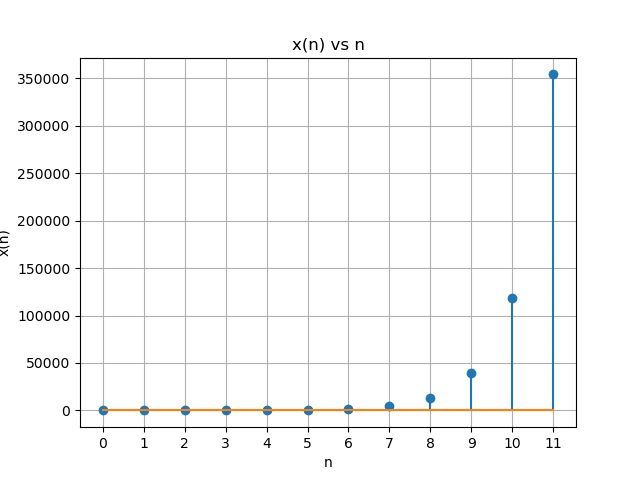
\includegraphics[width=1\linewidth]{/root/assign1/figs/figure__plot.png}
    \caption{plot x\brak{n}vs n\hspace{0.1cm}$p=486$,
    \hspace{0.1cm}$q=13122$,
    \hspace{0.1cm}$s=354294$,
    \hspace{0.1cm}$r=3$}
    \label{fig:1}
\end{figure}\\
\end{document}

\pagebreak
\item The sum of the first four terms of an A.P. is 56. The sum of the last four terms is
 112. If its first term is 11, then find the number of terms.\\
\solution
\iffalse
\let\negmedspace\undefined
\let\negthickspace\undefined
\documentclass[journal,12pt,twocolumn]{IEEEtran}
\usepackage{cite}
\usepackage{amsmath,amssymb,amsfonts,amsthm}
\usepackage{algorithmic}
\usepackage{graphicx}
\usepackage{textcomp}
\usepackage{xcolor}
\usepackage{txfonts}
\usepackage{listings}
\usepackage{enumitem}
\usepackage{mathtools}
\usepackage{gensymb}
\usepackage{comment}
\usepackage[breaklinks=true]{hyperref}
\usepackage{tkz-euclide} 
\use-package{listings}
\usepackage{gvv}                                        
\def\inputGnumericTable{}                                 
\usepackage[latin1]{inputenc}                                
\usepackage{color}                                            
\usepackage{array}                                            
\usepackage{longtable}                                       
\usepackage{calc}                                             
\usepackage{multirow}                                         
\usepackage{hhline}                                           
\usepackage{ifthen}                                           
\usepackage{lscape}
\usepackage{caption}

\newtheorem{theorem}{Theorem}[section]
\newtheorem{problem}{Problem}
\newtheorem{proposition}{Proposition}[section]
\newtheorem{lemma}{Lemma}[section]
\newtheorem{corollary}[theorem]{Corollary}
\newtheorem{example}{Example}[section]
\newtheorem{definition}[problem]{Definition}
\newcommand{\BEQA}{\begin{eqnarray}}
\newcommand{\EEQA}{\end{eqnarray}}
\newcommand{\define}{\stackrel{\triangle}{=}}
\theoremstyle{remark}
\newtheorem{rem}{Remark}
\begin{document}

\bibliographystyle{IEEEtran}
\vspace{3cm}

\title{11.9.5}
\author{EE23BTECH11029 - Kanishk}
\maketitle

\bigskip


\textbf{Question}:\\ 
The sum of the first four terms of an A.P. is 56. The sum of the last four terms is
112. If its first term is 11, then find the number of terms.\\

\textbf{Solution}:\\ 
\fi
\begin{table}[ht]
    \centering
    \def\arraystretch{1.5}
    \footnotesize
\begin{tabular}{|c|c|c|}
\hline
Symbol & Value & Description\\
\hline
$x(0)$ & $11$ & First term of AP \\
\hline
$y\brak{3}$ & $56$ & Sum of the first four terms of AP\\
\hline
$y\brak{n}-y\brak{n-4}$ & $112$& Sum of the last four terms of AP\\
\hline
\end{tabular}

   \caption{Input Parameters}
   \label{tab:11.9.5.12}
\end{table}

\small
\begin{align}
y\brak{n}&=\sbrak{\frac{\brak{n+1}}{2}\brak{2x\brak{0}+nd}}u\brak{n}\\
\implies y(3)&=\frac{4}{2}\brak{2x\brak{0}+3d}\\
\end{align}
From \tabref{tab:11.9.5.12}:
\begin{align}
\frac{4}{2}\brak{2x\brak{0}+3d}&=56\\
2x\brak{0}+3d&=28\\
\implies d&=2
\end{align}

\begin{align}
 y\brak{n}-y\brak{n-4}&=\frac{4}{2}\brak{2x\brak{n}+3\brak{-d}}
\end{align}
From \tabref{tab:11.9.5.12}:
\begin{align}
\frac{4}{2}\brak{2x\brak{n}+3\brak{-d}}&=112\\
2x\brak{n}-3d&=56\\
\implies x\brak{n}&=31\\
x\brak{0}+\brak{n}2&=31\\
\implies n&=10
\end{align}


\begin{align}
x\brak{n}&=\brak{x\brak{0}+2n}u\brak{n}\\
\implies X\brak{z}&=\frac{x\brak{0}}{1-z^{-1}}+2\frac{z^{-1}}{\brak{1-z^{-1}}^{2}}.\quad \abs{z} > 1
\end{align}

\newpage

\begin{figure}
    
    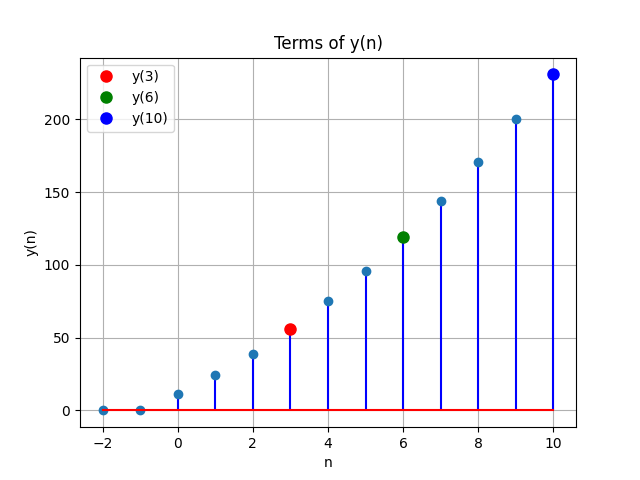
\includegraphics[width=\columnwidth]{ncert-maths/11/9/5/12//figs/fig1.png}
    \caption{Plot y(n) vs n}
\end{figure}

%\end{document}
\pagebreak
\item Find the sum to $n$ terms of the series whose $n^{th}$ term is given by $(2n-1)^2$ ? 
\solution
\iffalse
\let\negmedspace\undefined
\let\negthickspace\undefined
\documentclass[journal,12pt,onecolumn]{IEEEtran}
\usepackage{cite}
\usepackage{amsmath,amssymb,amsfonts,amsthm}
\usepackage{algorithmic}
\usepackage{graphicx}
\usepackage{textcomp}
\usepackage{xcolor}
\usepackage{txfonts}
\usepackage{listings}
\usepackage{enumitem}
\usepackage{mathtools}
\usepackage{gensymb}
\usepackage[breaklinks=true]{hyperref}
\usepackage{tkz-euclide} % loads  TikZ and tkz-base
\usepackage{listings}



\newtheorem{theorem}{Theorem}[section]
\newtheorem{problem}{Problem}
\newtheorem{proposition}{Proposition}[section]
\newtheorem{lemma}{Lemma}[section]
\newtheorem{corollary}[theorem]{Corollary}
\newtheorem{example}{Example}[section]
\newtheorem{definition}[problem]{Definition}
%\newtheorem{thm}{Theorem}[section] 
%\newtheorem{defn}[thm]{Definition}
%\newtheorem{algorithm}{Algorithm}[section]
%\newtheorem{cor}{Corollary}
\newcommand{\BEQA}{\begin{eqnarray}}
\newcommand{\EEQA}{\end{eqnarray}}
\newcommand{\system}[1]{\stackrel{#1}{\rightarrow}}
\newcommand{\define}{\stackrel{\triangle}{=}}
\theoremstyle{remark}
\newtheorem{rem}{Remark}
%\bibliographystyle{ieeetr}
\begin{document}
%
\providecommand{\pr}[1]{\ensuremath{\Pr\left(#1\right)}}
\providecommand{\prt}[2]{\ensuremath{p_{#1}^{\left(#2\right)} }}        % own macro for this question
\providecommand{\qfunc}[1]{\ensuremath{Q\left(#1\right)}}
\providecommand{\sbrak}[1]{\ensuremath{{}\left[#1\right]}}
\providecommand{\lsbrak}[1]{\ensuremath{{}\left[#1\right.}}
\providecommand{\rsbrak}[1]{\ensuremath{{}\left.#1\right]}}
\providecommand{\brak}[1]{\ensuremath{\left(#1\right)}}
\providecommand{\lbrak}[1]{\ensuremath{\left(#1\right.}}
\providecommand{\rbrak}[1]{\ensuremath{\left.#1\right)}}
\providecommand{\cbrak}[1]{\ensuremath{\left\{#1\right\}}}
\providecommand{\lcbrak}[1]{\ensuremath{\left\{#1\right.}}
\providecommand{\rcbrak}[1]{\ensuremath{\left.#1\right\}}}
\newcommand{\sgn}{\mathop{\mathrm{sgn}}}
\providecommand{\abs}[1]{\left\vert#1\right\vert}
\providecommand{\res}[1]{\Res\displaylimits_{#1}} 
\providecommand{\norm}[1]{\left\lVert#1\right\rVert}
%\providecommand{\norm}[1]{\lVert#1\rVert}
\providecommand{\mtx}[1]{\mathbf{#1}}
\providecommand{\mean}[1]{E\left[ #1 \right]}
\providecommand{\cond}[2]{#1\middle|#2}
\providecommand{\fourier}{\overset{\mathcal{F}}{ \rightleftharpoons}}
\newenvironment{amatrix}[1]{%
  \left(\begin{array}{@{}*{#1}{c}|c@{}}
}{%
  \end{array}\right)
}
%\providecommand{\hilbert}{\overset{\mathcal{H}}{ \rightleftharpoons}}
%\providecommand{\system}{\overset{\mathcal{H}}{ \longleftrightarrow}}
	%\newcommand{\solution}[2]{\textbf{Solution:}{#1}}
\newcommand{\solution}{\noindent \textbf{Solution: }}
\newcommand{\cosec}{\,\text{cosec}\,}
\providecommand{\dec}[2]{\ensuremath{\overset{#1}{\underset{#2}{\gtrless}}}}
\newcommand{\myvec}[1]{\ensuremath{\begin{pmatrix}#1\end{pmatrix}}}
\newcommand{\mydet}[1]{\ensuremath{\begin{vmatrix}#1\end{vmatrix}}}
\newcommand{\myaugvec}[2]{\ensuremath{\begin{amatrix}{#1}#2\end{amatrix}}}
\providecommand{\rank}{\text{rank}}
\providecommand{\pr}[1]{\ensuremath{\Pr\left(#1\right)}}
\providecommand{\qfunc}[1]{\ensuremath{Q\left(#1\right)}}
	\newcommand*{\permcomb}[4][0mu]{{{}^{#3}\mkern#1#2_{#4}}}
\newcommand*{\perm}[1][-3mu]{\permcomb[#1]{P}}
\newcommand*{\comb}[1][-1mu]{\permcomb[#1]{C}}
\providecommand{\qfunc}[1]{\ensuremath{Q\left(#1\right)}}
\providecommand{\gauss}[2]{\mathcal{N}\ensuremath{\left(#1,#2\right)}}
\providecommand{\diff}[2]{\ensuremath{\frac{d{#1}}{d{#2}}}}
\providecommand{\myceil}[1]{\left \lceil #1 \right \rceil }
\newcommand\figref{Fig.~\ref}
\newcommand\tabref{Table~\ref}
\newcommand{\sinc}{\,\text{sinc}\,}
\newcommand{\rect}{\,\text{rect}\,}
%%
%	%\newcommand{\solution}[2]{\textbf{Solution:}{#1}}
%\newcommand{\solution}{\noindent \textbf{Solution: }}
%\newcommand{\cosec}{\,\text{cosec}\,}
%\numberwithin{equation}{section}
%\numberwithin{equation}{subsection}
%\numberwithin{problem}{section}
%\numberwithin{definition}{section}
%\makeatletter
%\@addtoreset{figure}{problem}
%\makeatother

%\let\StandardTheFigure\thefigure
\let\vec\mathbf


\bibliographystyle{IEEEtran}
\title{SEQUENCE AND SERIES}
\author{EE23BTECH11011- Batchu Ishitha$^{*}$% <-this % stops a space
}
\maketitle




\bigskip

\renewcommand{\thefigure}{\theenumi}
\renewcommand{\thetable}{\theenumi}
%\renewcommand{\theequation}{\theenumi}

Q: Find the sum to $n$ terms of the series whose $n^{th}$ term is given by $(2n-1)^2$ ?

\solution
\fi
\begin{table}[!ht]
    \centering
        
      \begin{tabular}{|c|c|c|} 
      \hline
\textbf{Variable}& \textbf{Description}& \textbf{Value}\\\hline
         $x(n)$& $n^{th}$ term of sequence& $(2n+1)^2u(n)$\\\hline
          
    \end{tabular}


    \caption{input parameters}
    \label{}
\end{table}
Sum of $n$ terms of AP is given by
\begin{align}
 y(n)&=x(n)*u(n) \\
x(n)&= (2n+1)^2 u(n) 
\end{align}

\begin{equation}
   u(n) \xleftrightarrow{\mathcal{Z}} \frac{1}{(1-z^{-1})}  \quad \abs{z}>1\\ \label{eq:11.9.4.10.1.eq}
\end{equation}

\begin{equation}   
   nu(n) \xleftrightarrow{\mathcal{Z}} \frac{z^{-1}}{(1-z^{-1})^2} \quad \abs{z}>1\\ \label{eq:11.9.4.10.2.eq}
\end{equation}

\begin{equation}   
   n^2u(n) \xleftrightarrow{\mathcal{Z}} \frac{z^{-1}(1+z^{-1})}{(1-z^{-1})^3} \quad \abs{z}>1 \\ \label{eq:11.9.4.10.3.eq}
\end{equation}  

\begin{equation}
n^3u(n) \xleftrightarrow{\mathcal{Z}} \frac{z^{-1}\brak{1+4z^{-1}+z^{-2}}}{\brak{1-z^{-1}}^4} \quad \abs{z}>1 \\ \label{eq:11.9.4.10.4.eq}
\end{equation} 
 
\begin{align}
\implies  X(z)&=\frac{4z^{-1}(1+z^{-1})}{(1-z^{-1})^3} + \frac{1}{(1-z^{-1})} + \frac{4z^{-1}}{(1-z^{-1})^2} \quad \abs{z}>1 \\
 Y(z) &= X(z)U(z) \\
 &= \brak{\frac{4z^{-1}(z^{-1}+1)}{(1-z^{-1})^3} + \frac{1}{(1-z^{-1})} + \frac{4z^{-1}}{(1-z^{-1})^2}}\brak{\frac{1}{1-z^{-1}}}\\
 &= \frac{4z^{-1}(z^{-1}+1)}{(1-z^{-1})^4} + \frac{1}{(1-z^{-1})^2} + \frac{4z^{-1}}{(1-z^{-1})^3}
 \end{align}
 
 \begin{equation}
\implies Y(Z)=\frac{1}{(1-z^{-1})} +\frac{9z^{-1}}{(1-z^{-1})} + \frac{25z^{-2}}{(1-z^{-1})^2} + \frac{24z^{-3}}{(1-z^{-1})^3} + \frac{8z^{-4}}{(1-z^{-1})^4} \quad \abs{z}>1  \label{eq:11.9.4.10.5.eq}
 \end{equation}
Now from~\eqref{eq:11.9.4.10.1.eq},~\eqref{eq:11.9.4.10.2.eq},~\eqref{eq:11.9.4.10.3.eq},~\eqref{eq:11.9.4.10.4.eq},
 ~\eqref{eq:11.9.4.10.5.eq}
By using  inverse Z-transform pairs,
\begin{align}
  y\brak{n}&= u(n) + 9u(n-1) + 25(n-1)u(n-2) + 24\frac{(n-1)(n-2)}{2}u(n-3) + 8\frac{(n-1)(n-2)(n-3)}{6}u(n-4) \\
\implies  y\brak{n} &=\brak{\frac{4n^{3}+12n^{2}+11n+3}{3}}u(n)
\end{align}
$\therefore$ Sum of $n$ terms of the series whose $n^{th}$ term is given by $(2n+1)^2$ is $\frac{4n^{3}+12n^{2}+11n+3}{3}$  .
\begin{figure}[h]
    \centering
     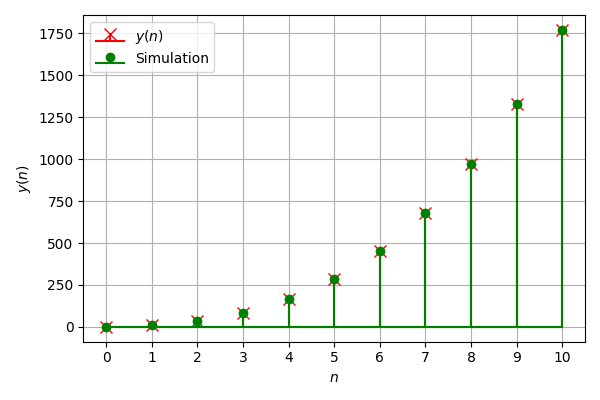
\includegraphics[width=\columnwidth]{ncert-maths/11/9/4/10/figs/fig2.png}
    \caption{Theory vs Simulation}    
    \label{}
\end{figure}


%\end{document}


\pagebreak
\item If the $4^{th}$, $10^{th}$ and $16^{th}$ terms of a G.P. are $x$, $y$, and $z$, respectively. Prove that $x,\; y,\; z$ are in G.P. \\
\solution
\iffalse
\let\negmedspace\undefined
\let\negthickspace\undefined
\documentclass[journal,12pt,twocolumn]{IEEEtran}
\usepackage{cite}
\usepackage{amsmath,amssymb,amsfonts,amsthm}
\usepackage{algorithmic}
\usepackage{graphicx}
\usepackage{textcomp}
\usepackage{xcolor}
\usepackage{txfonts}
\usepackage{listings}
\usepackage{enumitem}
\usepackage{mathtools}
\usepackage{gensymb}
\usepackage{comment}
\usepackage[breaklinks=true]{hyperref}
\usepackage{tkz-euclide} 
\usepackage{listings}
\usepackage{gvv}                                        
%\def\inputGnumericTable{}                                 
\usepackage[latin1]{inputenc}                                
\usepackage{color}                                            
\usepackage{array}                                            
\usepackage{longtable}                                       
\usepackage{calc}                                             
\usepackage{multirow}                                         
\usepackage{hhline}                                           
\usepackage{ifthen}                                           
\usepackage{lscape}
\usepackage{tabularx}
\usepackage{array}
\usepackage{float}


\newtheorem{theorem}{Theorem}[section]
\newtheorem{problem}{Problem}
\newtheorem{proposition}{Proposition}[section]
\newtheorem{lemma}{Lemma}[section]
\newtheorem{corollary}[theorem]{Corollary}
\newtheorem{example}{Example}[section]
\newtheorem{definition}[problem]{Definition}
\newcommand{\BEQA}{\begin{eqnarray}}
\newcommand{\EEQA}{\end{eqnarray}}
\newcommand{\define}{\stackrel{\triangle}{=}}
\theoremstyle{remark}
\newtheorem{rem}{Remark}
\begin{document}

\bibliographystyle{IEEEtran}
\vspace{3cm}

\title{11.9.3.17}
\author{EE23BTECH11017 - Eachempati Mihir Divyansh$^{*}$% <-this % stops a space
}
\maketitle
\newpage
\bigskip

\renewcommand{\thefigure}{\theenumi}
\renewcommand{\thetable}{\theenumi}

\textbf{Question: }
If the $4^{th}$, $10^{th}$ and $16^{th}$ terms of a G.P. are $x$, $y$, and $z$, respectively. Prove that $x,\; y,\; z$ are in G.P.
\\
\solution
\fi
\begin{table}[h]
    \centering
        \begin{tabular}{|m{2cm}|m{2cm}|m{2cm}|}
    \hline
    \textbf{Symbol} & \textbf{Value} & \textbf{Description}\\ [1ex]
    \hline
        $x$ & $x\brak{0}r^4$ & $x\brak{4}$ \\ [1ex]
    \hline
        $y$ & $x\brak{0}r^{10}$ & $x\brak{10}$\\ [1ex]
    \hline
        $z$ & $x\brak{0}r^{16}$ & $x\brak{16}$\\ [1ex]
    \hline
        $r$ & ? & $\frac{x\brak{n}}{x\brak{n-1}}$\\[1ex]
    \hline \vspace{0.1cm}
        $x\brak{0}$ & ? & First term \\[1ex]
    \hline
        $x\brak{n}$ & $x\brak{0}r^nu\brak{n}$ & General Term \\ [1ex]
    \hline
    \end{tabular}
\label{tab: 1}
                \caption{\textbf{Given Information}}
\end{table} 
\begin{enumerate}
\item From \tabref{tab: 1},
\begin{align}
    x&= x\brak{3} =x\brak{0}r^3 \\
	y&=x\brak{9}=x\brak{0}r^{9} \\
	z&=x\brak{15}=x\brak{0}r^{15}
\end{align}
Consider $\frac{x\brak{9}}{x\brak{3}}$ and $\frac{x\brak{15}}{x\brak{9}}$;
\begin{align}
	\frac{x\brak{9}}{x\brak{3}} &= \frac{x\brak{0}r^{9}}{x\brak{0}r^3} = r^6 = \frac{x\brak{15}}{x\brak{9}} = \frac{x\brak{0}r^{15}}{x\brak{0}r^{9}}\label{eqn: 4}
\end{align}
From \eqref{eqn: 4}, $x\brak{3}$, $x\brak{9}$, $x\brak{15}$ are in G.P.\\
$\therefore$  $x$, $y$, $z$ are in G.P.\\

\item
$x\brak{0}$ and $r$ can be expressed in terms of $x$, $y$, and $z$ in the following manner.
\begin{align}
    &\frac{y}{x}=r^6 \\
	\implies& r=\sqrt[6]{\frac{y}{x}}=\brak{\frac{y}{x}}^{\frac{1}{6}}\\
    \implies& x\brak{0}=\frac{x}{r^3} =x\brak{\frac{x}{y}}^{\frac{3}{6}}\\
	\therefore\; x\brak{0}&=x^{\frac{5}{3}}y^{-\frac{2}{3}}\;
	\text{and}\; r=\brak{\frac{y}{x}}^{\frac{1}{6}}= y^{\frac{1}{6}}x^{-\frac{1}{6}} \label{eqn: 8}
\end{align}
\item 
From \eqref{eq:gpz} Z-transform of a G.P. is
\begin{align}
    X\brak{z}&=\frac{x\brak{0}}{1-rz^{-1}}; \abs{z}>\abs{r}
\end{align}
Substituting $r$ and $x\brak{0}$ from \eqref{eqn: 8}, 
\begin{align}
     X\brak{z}&=\frac{x^{\frac{5}{3}}y^{-\frac{2}{3}}}{1-{\brak{\frac{y}{x}}^{\frac{1}{6}}}z^{-1}}
\end{align}
\item Example 
Let $x(0)=1$ and $r=1.2$
\begin{align}
    x=x\brak{3}=& \brak{1.2}^3 \\
    y=x\brak{9}=&=\brak{1.2}^9\\
    z=x\brak{15}=&\brak{1.2}^{15}
\end{align}
\begin{figure}[h]
    \centering
    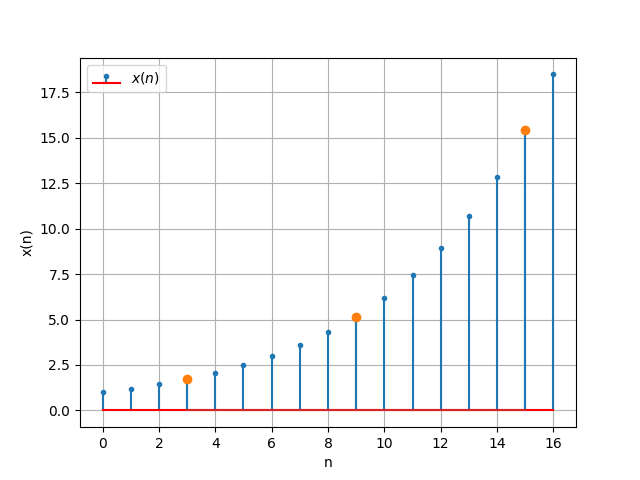
\includegraphics[width=\columnwidth]{ncert-maths/11/9/3/17/figs/A_1.png}
	\caption{Stem Plot of $x(n)$ vs $n$}
        \label{fig:1}
\end{figure}


\end{enumerate}


\pagebreak
\item Show that the ratio of the sum of the first \(n\) terms of a geometric progression (G.P.) to the sum of terms from \((n+1)\)th to \((2n)\)th term is \(\frac{1}{r^n}\).
\solution
\pagebreak
\item A G.P consists of an even number of terms. If the sum of all terms is 5 times the sum of terms occupying odd places, then find its common ratio.\\
\solution
\documentclass[journal,12pt,twocolumn]{IEEEtran}
\usepackage{cite}
\usepackage{amsmath,amssymb,amsfonts,amsthm}
\usepackage{algorithmic}
\usepackage{graphicx}
\usepackage{textcomp}
\usepackage{xcolor}
\usepackage{txfonts}
\usepackage{listings}
\usepackage{enumitem}
\usepackage{mathtools}
\usepackage{gensymb}
\usepackage{comment}
\usepackage[breaklinks=true]{hyperref}
\usepackage{tkz-euclide}
\usepackage{gvv}
\def\inputGnumericTable{}
\usepackage[latin1]{inputenc}
\usepackage{color}
\usepackage{array}
\usepackage{longtable}
\usepackage{calc}
\usepackage{multirow}
\usepackage{hhline}
\usepackage{ifthen}
\usepackage{lscape}

\newtheorem{theorem}{Theorem}[section]
\newtheorem{problem}{Problem}
\newtheorem{proposition}{Proposition}[section]
\newtheorem{lemma}{Lemma}[section]
\newtheorem{corollary}[theorem]{Corollary}
\newtheorem{example}{Example}[section]
\newtheorem{definition}[problem]{Definition}
\newcommand{\BEQA}{\begin{eqnarray}}
\newcommand{\EEQA}{\end{eqnarray}}
\newcommand{\define}{\stackrel{\triangle}{=}}
\theoremstyle{remark}
\newtheorem{rem}{Remark}
\begin{document}

\bibliographystyle{IEEEtran}
\title{Maths Assignment}
\author{Abhignya Gogula\\
        EE23BTECH11023}
\maketitle
\section*{Problem Statement}
A G.P consists of an even number of terms. If the sum of all terms is 5 times the sum of terms occupying odd places, then find its common ratio.
\section*{Solution}
\begin{table}[h!]
\centering
\begin{table}[h]
\renewcommand\thetable{1}
    \centering
    \begin{tabular}{|c|c|c|}
        \hline
        \textbf{Parameter} & \textbf{Description} & \textbf{Value}\\
        \hline
        $x(0)$ & First term & $2$\\
        \hline
        $x(19)$ & $20\textsuperscript{th}$ term & $-112$\\
        \hline
        $y(n)$ & sum upto $n\textsuperscript{th}$ term & \\
        \hline
    \end{tabular}
    \caption{Input data}
  \label{input data}
\end{table}

\caption{Input Parameters}
\label{11.9.5.11tab1}
\end{table}
Solving the Question in time domain:
\begin{align}
x(n) &= x(0)r^{n} \\
y(n) &= x(0)\brak{\frac{r^{n+1}-1}{r-1}}u(n)
\label{eq:11.9.5.11eq1}
\end{align}
The sum of terms in odd places:
\begin{align}
x_o(n) &= x(0)r^{2n}
\end{align}
\begin{equation}
y_o(n)= x(0)\brak{\frac{r^{n+1}-1}{r^2-1}}u(n)
\label{eq:11.9.5.11eq2}
\end{equation}
Then from \eqref{eq:11.9.5.11eq1} and \eqref{eq:11.9.5.11eq2}
\begin{align}
x(0)\brak{\frac{r^{N}-1}{r-1}}u(n) &= 5\brak{x(0)\brak{\frac{r^{2M}-1}{r^2-1}}u(n)}\\
\frac{r^2-1}{r-1} &= 5\\
\text{as } r \neq 1, \quad \text{hence } r &= 4\\
\end{align}
X,Y,Xo,Yo are frequency counterparts of the above GP
\begin{align}
X(z) &= \frac{x(0)}{1-rz^{-1}} \quad \abs{z} > \abs{r}\\ 
X_o(z) &= \frac{x(0)}{1-r^{2}z^{-1}}\\
Y(z) &= \frac{x(0)}{\brak{1-rz^{-1}}\brak{1-z^{-1}}}\\
Y_o(z) &= \frac{x(0)}{\brak{1-rz^{\frac{-1}{2}}}\brak{1-z^{-1}}}
\end{align}
\end{document}


\pagebreak
\item Find the sum to indicated number of terms in the geometric progression $x^3,x^5,x^7,...n$ terms (if $x\neq\pm1$).\\
\solution
\iffalse
\let\negmedspace\undefined
\let\negthickspace\undefined
\documentclass[journal,12pt,twocolumn]{IEEEtran}
\usepackage{cite}
\usepackage{amsmath,amssymb,amsfonts,amsthm}
\usepackage{algorithmic}
\usepackage{graphicx}
\usepackage{textcomp}
\usepackage{xcolor}
\usepackage{txfonts}
\usepackage{listings}
\usepackage{enumitem}
\usepackage{mathtools}
\usepackage{gensymb}
\usepackage{comment}
\usepackage[breaklinks=true]{hyperref}
\usepackage{tkz-euclide} 
\usepackage{listings}
\usepackage{gvv}                                        
\def\inputGnumericTable{}                                 
\usepackage[latin1]{inputenc}                                
\usepackage{color}                                            
\usepackage{array}                                            
\usepackage{longtable}                                       
\usepackage{calc}                                             
\usepackage{multirow}                                         
\usepackage{hhline}                                           
\usepackage{ifthen}                                           
\usepackage{lscape}
\newtheorem{theorem}{Theorem}[section]
\newtheorem{problem}{Problem}
\newtheorem{proposition}{Proposition}[section]
\newtheorem{lemma}{Lemma}[section]
\newtheorem{corollary}[theorem]{Corollary}
\newtheorem{example}{Example}[section]
\newtheorem{definition}[problem]{Definition}
\newcommand{\BEQA}{\begin{eqnarray}}
\newcommand{\EEQA}{\end{eqnarray}}
\newcommand{\define}{\stackrel{\triangle}{=}}
\theoremstyle{remark}
\newtheorem{rem}{Remark}
\begin{document}

\bibliographystyle{IEEEtran}
\vspace{3cm}

\title{NCERT 11.9.3.Q10}
\author{EE23BTECH11224 - Sri Krishna Prabhas Yadla$^{*}$% <-this % stops a space
}
\maketitle
\newpage
\bigskip

\renewcommand{\thefigure}{\arabic{figure}}
\renewcommand{\thetable}{\arabic{table}}


\vspace{3cm}
\textbf{Question:} Find the sum to indicated number of terms in the geometric progression $x^3,x^5,x^7,...n$ terms (if $x\neq\pm1$).
\\
\solution
\fi
\begin{table}[htbp]
\centering
\def\arraystrech{1.5}
	\begin{tabular}{|c|c|c|}
\hline
		\textbf{Input Parameters} & \textbf{Values} & \textbf{Description} \\
\hline
		$x(0)$ & $x^3$ & Initial term\\
\hline
		$r$ & $x^2$ & Common ratio\\
\hline
		$x(n)$ & $x^{2n+3}u(n)$ & General term \\
\hline
\end{tabular}
\caption{Given inputs}
\label{tab:1.11.9.3.Q10}
\end{table}

\newline
From \tabref{tab:1.11.9.3.Q10},
\begin{align}
	X(z) &= \frac{x(0)}{1-rz^{-1}} \\
	&= \frac{x^3}{1-x^2z^{-1}} \quad \abs{z}>x^2 \\
	y(n) &= x(n) * u(n) \\
	Y(z) &= X(z)U(z) \\
	&= \frac{x^3}{(1-x^2z^{-1})(1-z^{-1})} \quad  \abs{z} > x^2 \cap \abs{z}>1\\
	&= \frac{x^3}{x^2-1}\brak{\frac{x^2}{1-x^2z^{-1}}-\frac{1}{1-z^{-1}}} \\
	u(n) &\system{Z} \frac{1}{1-z^{-1}} \quad \abs{z}>1 \\
	x^{2n+2} u(n) &\system{Z} \frac{x^2}{1-x^2z^{-1}} \quad \abs{z}>x^2
\end{align}
Taking inverse Z transform of $Y(z)$,
\begin{align}
	y(n) &= x^3\brak{\frac{x^{2n+2}-1}{x^2-1}}u(n)
\end{align}
\begin{figure}[ht!]
	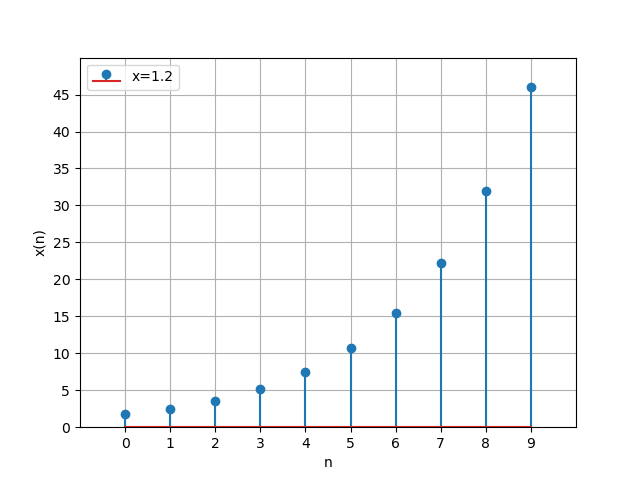
\includegraphics[width=\columnwidth]{ncert-maths/11/9/3/10/figs/plot_2.png}
	\caption{Plot of $x(n)$ for $x=1.2$}
	\label{fig:1.2}
\end{figure}

\pagebreak
\item Determine the AP whose third term is 16 and the 7th term exceeds the 5th term by 12. \\
\solution
\documentclass[12pt]{article}
\usepackage{amsmath}
\usepackage{graphicx}
\usepackage{float}
\usepackage{amssymb}
\usepackage{pgfplots}
\pgfplotsset{compat=1.18}
\newcommand{\tabref}[1]{Table~\ref{#1}}
\newcommand{\figref}[1]{Figure~\ref{#1}}
\providecommand{\abs}[1]{\left\vert#1\right\vert}

\begin{document}

\title{Discrete Assignment}
\author{Mohana Eppala\\ EE23BTECH11018}
\maketitle

\section*{Problem Statement}
Determine the AP whose third term is 16 and the 7th term exceeds the 5th term by 12. 
\section*{Solution}
\begin{table}[H]

\centering
\begin{tabular}{|c|c|c|}
        \hline
        \textbf{Parameter} & \textbf{Value} & \textbf{Description} \\
        \hline
        $x(6) - x(4)$ & 12 & 7th term exceeds 5th by 12 \\
        \hline
	$x(2)$ & 16 & Third term \\
	\hline
        $d$ & ? & Common difference \\
        \hline
        $x(0)$ & ? & First term of AP \\
	\hline
        $x(n)$ & $(x(0) + nd)u(n)$ & General term \\
        \hline
\end{tabular}
\caption{Input parameters table}
\label{tab:1}

\end{table}


From \tabref{tab:1}
\begin{align}
    x(0) +6d - x(0) - 4d &= 12 \\ \implies
    2d &= 12\\ \implies
    d &= 6
\end{align}
Also,
\begin{align}
     x(0) + 2d &= 16 \\ \implies
	x(0) + 2(6) &= 16 \\ \implies
	x(0) &= 4 \\
	\therefore x(n) &= 6n + 4 
\end{align}
From \tabref{tab:1}
\begin{align}
	X(z) &= x(0)  \frac{1}{1-z^{-1}} + d \frac{z^{-1}}{(1 - z^{-1})^2} \\
	&= 4 \frac{1}{1-z^{-1}} + 6 \frac{z^{-1}}{(1 - z^{-1})^2} \\
	&= \frac{4+2z^{-1}}{(1-z^{-1})^2} \quad \abs{z} > 1
\end{align}



\begin{figure}[H]
    \centering
    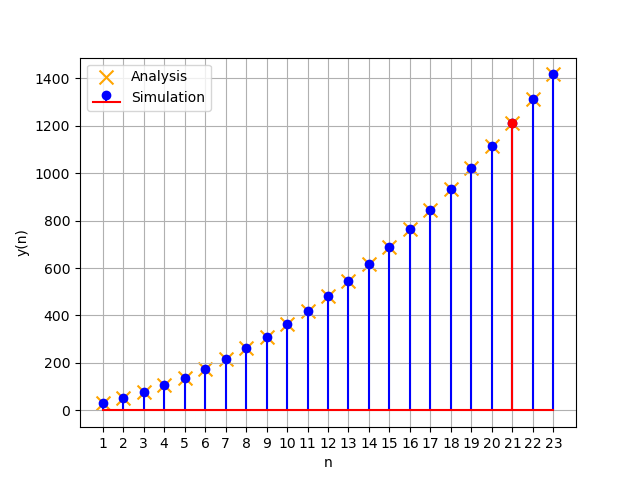
\includegraphics{figs/fig1.png}
    \caption{Given AP}
    \label{fig}
\end{figure}

\end{document}


\pagebreak
\item Find the seventh term of the sequence where the nth term is given by $a_n= \frac {n^2}{2^{n}}$\\
\solution

\iffalse
\documentclass[journal,12pt,twocolumn]{IEEEtran}
\usepackage{cite}
\usepackage{amsmath,amssymb,amsfonts,amsthm}
\usepackage{algorithmic}
\usepackage{graphicx}
\usepackage{textcomp}
\usepackage{xcolor}
\usepackage{txfonts}
\usepackage{listings}
\usepackage{enumitem}
\usepackage{mathtools}
\usepackage{float}
\usepackage{gensymb}
\usepackage{comment}
\usepackage[breaklinks=true]{hyperref}
\usepackage{tkz-euclide} 
\usepackage{listings}
\usepackage{gvv}                                        
\def\inputGnumericTable{}                                 
\usepackage[latin1]{inputenc}                                
\usepackage{color}                                            
\usepackage{array}                                            
\usepackage{longtable}                                       
\usepackage{calc}                                             
\usepackage{multirow}                                         
\usepackage{hhline}                                           
\usepackage{ifthen}                                           
\usepackage{lscape}
\usepackage{amsmath}
\newtheorem{theorem}{Theorem}[section]
\newtheorem{problem}{Problem}
\newtheorem{proposition}{Proposition}[section]
\newtheorem{lemma}{Lemma}[section]
\newtheorem{corollary}[theorem]{Corollary}
\newtheorem{example}{Example}[section]
\newtheorem{definition}[problem]{Definition}
\newcommand{\BEQA}{\begin{eqnarray}}
\newcommand{\EEQA}{\end{eqnarray}}
\newcommand{\define}{\stackrel{\triangle}{=}}
\theoremstyle{remark}
\newtheorem{rem}{Remark}

\begin{document}

\bibliographystyle{IEEEtran}
\vspace{3cm}

\title{NCERT Discrete - 11.9.1.8}
\author{EE23BTECH11045 - Palavelli Srija$^{*}$}

\maketitle
\newpage
\bigskip

\renewcommand{\thefigure}{\theenumi}
\renewcommand{\thetable}{\theenumi}

\vspace{3cm}
\textbf{Question 11.9.1.8:} 
\begin{enumerate}
\item Find the seventh term of the sequence where the nth term is given by $a_n= \frac {n^2}{2^{n}}$
\end{enumerate}

\textbf{Solution: }
\fi
\begin{align}
 x(n) &= \frac{(n+1)^2}{2^{(n+1)}}u(n)
\end{align}

\begin{table}[h!]
    \centering
     \begin{tabular}{|c|c|}
        \hline
        \textbf{Parameter} & \textbf{Value} \\
        \hline
        \(x(n)\) & \(\frac{(n+1)^2}{2^(n+1)}u(n)\) \\ \\
        \(x(6)\) & ? \\
        \hline
    \end{tabular}

    \caption{Input Parameters}
    \label{tab:table_sr}
\end{table}

\begin{align}
x(6) &= \frac{(6+1)^2}{2^{(6+1)}}\\
     &= \frac {49}{128}
\end{align}

\begin{enumerate}
   \item Scaling property:
     \begin{align}
         a^{n} u(n) & \xleftrightarrow{\mathcal{Z}}  \frac{1}{(1-az^{-1})}, \quad \lvert z \rvert > \lvert a \rvert 
     \end{align}
     
   \item Differentiation property:
    \begin{align}
     n u(n) & \xleftrightarrow{\mathcal{Z}} (-z) \frac{dY(z)}{dz} \\
     \implies n u(n) & \xleftrightarrow{\mathcal{Z}}  \frac{z^{-1}}{(1-z^{-1})^2}, \quad \lvert z \rvert > 1 \\
     \implies n^2 u(n) & \xleftrightarrow{\mathcal{Z}}  \frac{z^{-1}(1+z^{-1})}{(1-z^{-1})^3}, \quad \lvert z \rvert > 1
   \end{align}
   
   \item Time shifting property:
    \begin{align}
         y(n-k) & \xleftrightarrow{\mathcal{Z}} z^{-k}Y(z)
     \end{align}
\end{enumerate}

The Z transform of $x(n)$ is given by:\\
from(4)
\begin{align}
\frac{u(n)}{2^n} & \xleftrightarrow{\mathcal{Z}}  \frac{1}{(1-(2z)^{-1})}, \quad \lvert z \rvert>\frac{1}{2}
\end{align}
	from(5)
\begin{align}
\frac{n}{2^n} u(n) & \xleftrightarrow{\mathcal{Z}} \frac{(2z)^{-1}}{(1-(2z)^{-1})^2}, \quad \lvert z \rvert>\frac{1}{2}\\
\frac{n^2}{2^n} u(n) & \xleftrightarrow{\mathcal{Z}} \frac{(2z)^{-1}(1 + (2z)^{-1})}{(1 - (2z)^{-1})^3}, \quad \lvert z \rvert>\frac{1}{2}
\end{align}
	from(8)
\begin{align}
\frac{(n+1)^2}{2^(n+1)} u(n) & \xleftrightarrow{\mathcal{Z}} (z) \frac{(2z)^{-1}(1 + (2z)^{-1})}{(1 - (2z)^{-1})^3}, \quad \lvert z \rvert > \frac{1}{2}
\end{align}

\begin{align}
X(z) &= \frac{1 + (2z)^{-1}}{2(1 - (2z)^{-1})^3}, \quad \lvert z \rvert > \frac{1}{2}
\end{align}

\begin{figure}[h!]
    \centering
    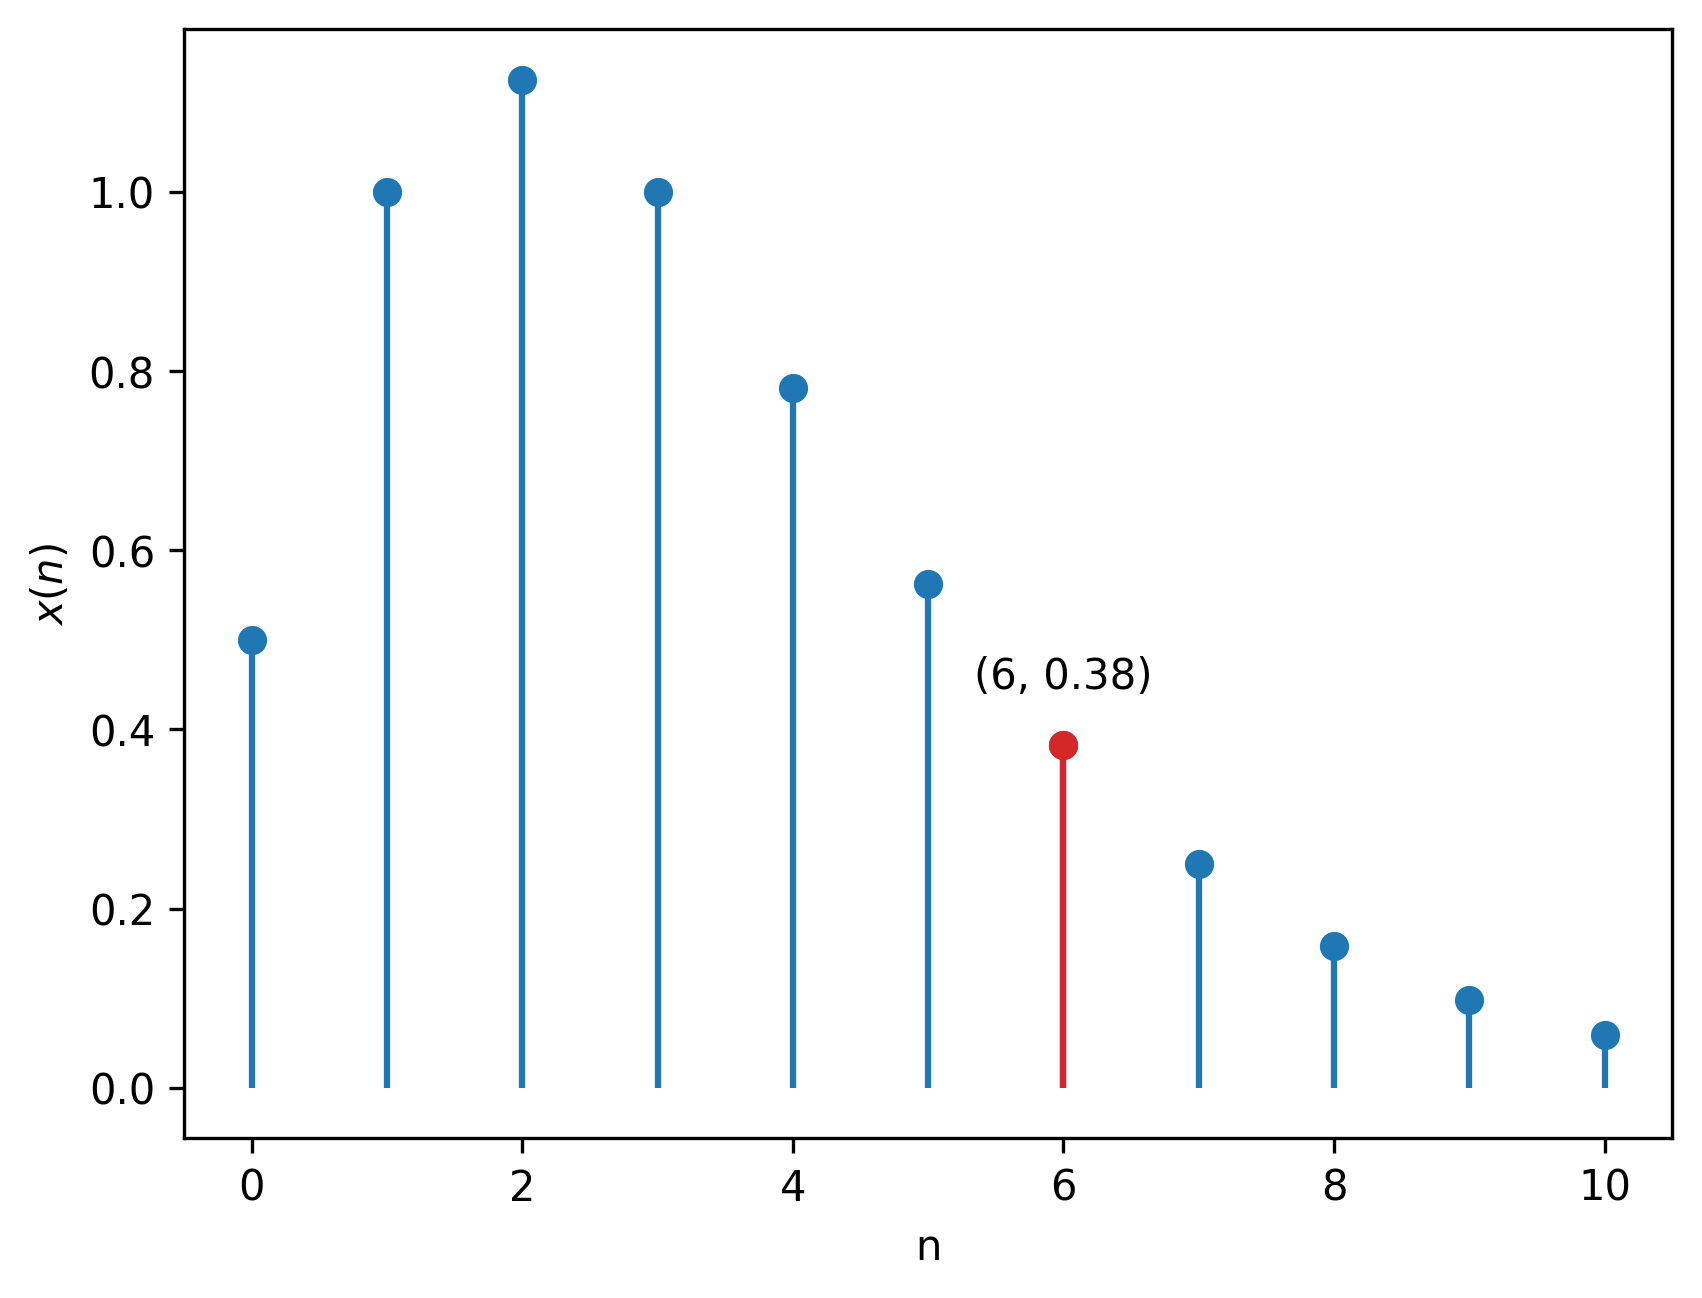
\includegraphics[width=\columnwidth]{ncert-maths/11/9/1/8/figs/plot.png}
    \caption{Stem plot of $x(n)$}
    \label{fig:sr1}
\end{figure}

%\end{document}

\pagebreak
\item Find sum to n terms of the following series:\\
$\frac{1}{1 \times 2} + \frac{1}{2 \times 3} + \frac{1}{3 \times 4} + \ldots$ \hfill(NCERT 11.9.4.4)
\solution
\pagebreak
\item 1x2x3 + 2x3x4 + 3x4x5 +..... \\
\solution
\pagebreak
\item  Find the sum of the following series up to \(n\) terms:
          \begin{enumerate}
              \item $5 + 55 + 555 + \ldots$
              \item  $.6 + .66 + .666 + \ldots$
        \end{enumerate}

\solution
\pagebreak
\item Find $a_{9}$ in the sequence $a_{n}=\brak{-1}^{n-1}n^{3}$ \\
\solution
\pagebreak
\item Find the 20th term in this series.\\
$$2\times4+4\times6+6\times8\cdots+n\,terms$$ \\
\solution
\pagebreak

\item Q10) The sum of three numbers in G.P. is 56. If we subtract 1, 7, 21 from these numbers in that order, we obtain an arithmetic progression. Find the numbers.\\
\solution
\item  Find the sum to n terms for the given series: $3\times8 + 6\times11 + 9\times14 + ...$
\solution
\pagebreak
\item Find the sum to $n$ terms of the series:\\
$1^2+\brak{1^2+2^2}+\brak{1^2+2^2+3^2}+...$ \hfill(NCERT 11.9.4.7)\\
\solution
\iffalse
\let\negmedspace\undefined
\let\negthickspace\undefined
\documentclass[journal,12pt,twocolumn]{IEEEtran}
\usepackage{cite}
\usepackage{amsmath,amssymb,amsfonts,amsthm}
\usepackage{algorithmic}
\usepackage{graphicx}
\usepackage{textcomp}
\usepackage{xcolor}
\usepackage{txfonts}
\usepackage{listings}
\usepackage{enumitem}
\usepackage{mathtools}
\usepackage{gensymb}
\usepackage{comment}
\usepackage[breaklinks=true]{hyperref}
\usepackage{tkz-euclide} 
\usepackage{listings}
\usepackage{gvv}                                        
\def\inputGnumericTable{}                                 
\usepackage[latin1]{inputenc}                                
\usepackage{color}                                            
\usepackage{array}                                            
\usepackage{longtable}                                       
\usepackage{calc}                                             
\usepackage{multirow}                                         
\usepackage{hhline}                                           
\usepackage{ifthen}                                           
\usepackage{lscape}
\newtheorem{theorem}{Theorem}[section]
\newtheorem{problem}{Problem}
\newtheorem{proposition}{Proposition}[section]
\newtheorem{lemma}{Lemma}[section]
\newtheorem{corollary}[theorem]{Corollary}
\newtheorem{example}{Example}[section]
\newtheorem{definition}[problem]{Definition}
\newcommand{\BEQA}{\begin{eqnarray}}
\newcommand{\EEQA}{\end{eqnarray}}
\newcommand{\define}{\stackrel{\triangle}{=}}
\theoremstyle{remark}
\newtheorem{rem}{Remark}
\begin{document}

\bibliographystyle{IEEEtran}
\vspace{3cm}

\title{11.9.4.7}
\author{EE23BTECH11063 - Vemula Siddhartha
}
\maketitle
\newpage
\bigskip

\renewcommand{\thefigure}{\theenumi}
\renewcommand{\thetable}{\theenumi}
\textbf{Question}:\\
Find the sum to $n$ terms of the series:\\
    $1^2+\brak{1^2+2^2}+\brak{1^2+2^2+3^2}+...$
    \\
\textbf{Solution:}
\fi
\begin{table}[h!]    
    \centering
    \begin{tabular}[12pt]{ |c| c| c|}
    \hline
    \textbf{Variable} & \textbf{Description}&\textbf{Value}\\ 
    \hline
    $y\brak{n}$ & Sum of $n+1$ terms of the series&?\\
    \hline
    $x\brak{n}$ & General term& $\brak{n+1}^2u\brak{n}$\\
    \hline   
    \end{tabular}
    \caption{Variables Used}
    \label{tab:11.9.4.7.1}
  \end{table}
\begin{align}
    y\brak{n}&=1^2+\brak{1^2+2^2}+\brak{1^2+2^2+3^2}+...
\end{align}
Let,
\begin{align}
    x\brak{n}&=\brak{n+1}^2u\brak{n}\\
    \implies y\brak{n}&=x\brak{n}*u\brak{n}*u\brak{n}\\
    Y\brak{z}&=X\brak{z}\brak{U\brak{z}}^2
\end{align}
From \eqref{eq:11.9.5.26.3},
\begin{align}
    n^2u\brak{n}\system{Z}\frac{z^{-1}\brak{1+z^{-1}}}{\brak{1-z^{-1}}^3}\;\;\cbrak{\abs{z}>1}
\end{align}
Using \eqref{eq:shiftk},
\begin{align}
    \brak{n+1}^2u\brak{n}&\system{Z}\frac{1+z^{-1}}{\brak{1-z^{-1}}^3}\;\;\cbrak{\abs{z}>1}\label{eq:11.9.4.7.1}
\end{align}
From \eqref{eq:11.9.4.7.1},
\begin{align}
    Y\brak{z}&=\brak{\frac{1+z^{-1}}{\brak{1-z^{-1}}^3}}\brak{\frac{1}{1-z^{-1}}}^2\\
    &=\frac{1+z^{-1}}{\brak{1-z^{-1}}^5}\\
    &=\frac{1}{\brak{1-z^{-1}}^5}+\frac{z^{-1}}{\brak{1-z^{-1}}^5}\;\cbrak{\abs{z}>1}
\end{align}
From \eqref{eq:11.9.5.26.12}, using \eqref{eq:shiftk},
\begin{align}
    \frac{\brak{n+1}\brak{n+2}\brak{n+3}\brak{n+4}}{24}u\brak{n}&\system{Z}\frac{1}{\brak{1-z^{-1}}^5}\label{eq:11.9.4.7.2}\cbrak{\abs{z}>1}\\
    \frac{\brak{n}\brak{n+1}\brak{n+2}\brak{n+3}}{24}u\brak{n}&\system{Z}\frac{z^{-1}}{\brak{1-z^{-1}}^5}\label{eq:11.9.4.7.3}\cbrak{\abs{z}>1}
\end{align}
From \eqref{eq:11.9.4.7.2} and \eqref{eq:11.9.4.7.3}, taking the Inverse Z Transform,
\begin{align}
    y\brak{n}&=\brak{\frac{\brak{n+1}\brak{n+2}\brak{n+3}\brak{n+4}}{24}u\brak{n}}\notag\\
    &\;+\brak{\frac{\brak{n}\brak{n+1}\brak{n+2}\brak{n+3}}{24}u\brak{n}}\\
    \implies y\brak{n}&=\frac{\brak{n+1}\brak{n+2}^2\brak{n+3}}{12}u\brak{n}
\end{align}
\begin{figure}[h!]
    \centering
    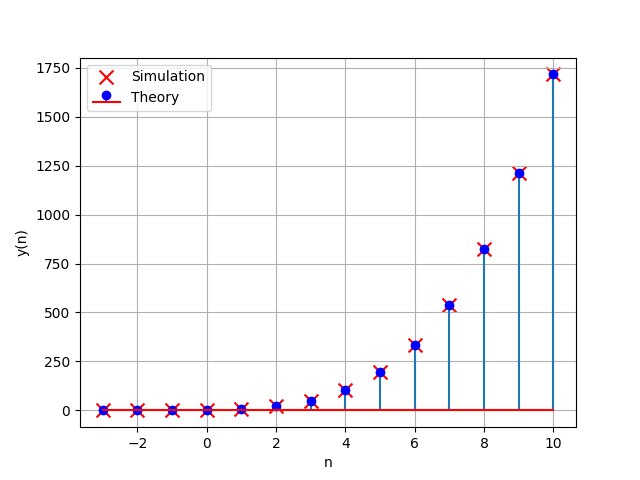
\includegraphics[width=\linewidth]{ncert-maths/11/9/4/7/figs/Figure_1.png}
    \caption{Stem Plot of $y\brak{n}$}
\end{figure}

\pagebreak
\item Find a GP for which sum of the first two terms is -4 and the fifth term is 4 times the third term.\\
\solution
\iffalse
\let\negmedspace\undefined
\let\negthickspace\undefined
\documentclass[journal,12pt,twocolumn]{IEEEtran}
\usepackage{cite}
\usepackage{amsmath,amssymb,amsfonts,amsthm}
\usepackage{algorithmic}
\usepackage{graphicx}
\usepackage{textcomp}
\usepackage{xcolor}
\usepackage{txfonts}
\usepackage{listings}
\usepackage{enumitem}
\usepackage{mathtools}
\usepackage{gensymb}
\usepackage{comment}
\usepackage[breaklinks=true]{hyperref}
\usepackage{tkz-euclide} % loads  TikZ and tkz-base
\usepackage{listings}
\usepackage[latin1]{inputenc}                                
\usepackage{color}                                            
\usepackage{array}                                            
\usepackage{longtable}                                       
\usepackage{calc}                                             
\usepackage{multirow}                                         
\usepackage{hhline}                                           
\usepackage{ifthen}                                           
\usepackage{lscape}
\usepackage{caption}
\usepackage{subcaption}


\newtheorem{theorem}{Theorem}[section]
\newtheorem{problem}{Problem}
\newtheorem{proposition}{Proposition}[section]
\newtheorem{lemma}{Lemma}[section]
\newtheorem{corollary}[theorem]{Corollary}
\newtheorem{example}{Example}[section]
\newtheorem{definition}[problem]{Definition}
%\newtheorem{thm}{Theorem}[section] 
%\newtheorem{defn}[thm]{Definition}
%\newtheorem{algorithm}{Algorithm}[section]
%\newtheorem{cor}{Corollary}
\newcommand{\BEQA}{\begin{eqnarray}}
\newcommand{\EEQA}{\end{eqnarray}}
\newcommand{\define}{\stackrel{\triangle}{=}}
\theoremstyle{remark}
\newtheorem{rem}{Remark}
%\bibliographystyle{ieeetr}

\begin{document}

%
\providecommand{\pr}[1]{\ensuremath{\Pr\left(#1\right)}}
\providecommand{\prt}[2]{\ensuremath{p_{#1}^{\left(#2\right)} }}        % own macro for this question
\providecommand{\qfunc}[1]{\ensuremath{Q\left(#1\right)}}
\providecommand{\sbrak}[1]{\ensuremath{{}\left[#1\right]}}
\providecommand{\lsbrak}[1]{\ensuremath{{}\left[#1\right.}}
\providecommand{\rsbrak}[1]{\ensuremath{{}\left.#1\right]}}
\providecommand{\brak}[1]{\ensuremath{\left(#1\right)}}
\providecommand{\lbrak}[1]{\ensuremath{\left(#1\right.}}
\providecommand{\rbrak}[1]{\ensuremath{\left.#1\right)}}
\providecommand{\cbrak}[1]{\ensuremath{\left\{#1\right\}}}
\providecommand{\lcbrak}[1]{\ensuremath{\left\{#1\right.}}
\providecommand{\rcbrak}[1]{\ensuremath{\left.#1\right\}}}
\newcommand{\sgn}{\mathop{\mathrm{sgn}}}
\providecommand{\abs}[1]{\left\vert#1\right\vert}
\providecommand{\res}[1]{\Res\displaylimits_{#1}} 
\providecommand{\norm}[1]{\left\lVert#1\right\rVert}
%\providecommand{\norm}[1]{\lVert#1\rVert}
\providecommand{\mtx}[1]{\mathbf{#1}}
\providecommand{\mean}[1]{E\left[ #1 \right]}
\providecommand{\cond}[2]{#1\middle|#2}
\providecommand{\fourier}{\overset{\mathcal{F}}{ \rightleftharpoons}}
\newenvironment{amatrix}[1]{%
  \left(\begin{array}{@{}*{#1}{c}|c@{}}
}{%
  \end{array}\right)
}
%\providecommand{\hilbert}{\overset{\mathcal{H}}{ \rightleftharpoons}}
%\providecommand{\system}{\overset{\mathcal{H}}{ \longleftrightarrow}}
        %\newcommand{\solution}[2]{\textbf{Solution:}{#1}}
\newcommand{\solution}{\noindent \textbf{Solution: }}
\newcommand{\cosec}{\,\text{cosec}\,}
\providecommand{\dec}[2]{\ensuremath{\overset{#1}{\underset{#2}{\gtrless}}}}
\newcommand{\myvec}[1]{\ensuremath{\begin{pmatrix}#1\end{pmatrix}}}
\newcommand{\mydet}[1]{\ensuremath{\begin{vmatrix}#1\end{vmatrix}}}
\newcommand{\myaugvec}[2]{\ensuremath{\begin{amatrix}{#1}#2\end{amatrix}}}
\providecommand{\rank}{\text{rank}}
\providecommand{\pr}[1]{\ensuremath{\Pr\left(#1\right)}}
\providecommand{\qfunc}[1]{\ensuremath{Q\left(#1\right)}}
        \newcommand*{\permcomb}[4][0mu]{{{}^{#3}\mkern#1#2_{#4}}}
\newcommand*{\perm}[1][-3mu]{\permcomb[#1]{P}}
\newcommand*{\comb}[1][-1mu]{\permcomb[#1]{C}}
\providecommand{\qfunc}[1]{\ensuremath{Q\left(#1\right)}}
\providecommand{\gauss}[2]{\mathcal{N}\ensuremath{\left(#1,#2\right)}}
\providecommand{\diff}[2]{\ensuremath{\frac{d{#1}}{d{#2}}}}
\providecommand{\myceil}[1]{\left \lceil #1 \right \rceil }
\newcommand\figref{Fig.~\ref}
\newcommand\tabref{Table~\ref}
\newcommand{\sinc}{\,\text{sinc}\,}
\newcommand{\rect}{\,\text{rect}\,}
%%
%       %\newcommand{\solution}[2]{\textbf{Solution:}{#1}}
%\newcommand{\solution}{\noindent \textbf{Solution: }}
%\newcommand{\cosec}{\,\text{cosec}\,}
%\numberwithin{equation}{section}
%\numberwithin{equation}{subsection}
%\numberwithin{problem}{section}
%\numberwithin{definition}{section}
%\makeatletter
%\@addtoreset{figure}{problem}
%\makeatother

%\let\StandardTheFigure\thefigure
\let\vec\mathbf

\bibliographystyle{IEEEtran}

\vspace{3cm}
\title{Assignment}
\author{EE23BTECH11001 - Aashna Sahu}
\maketitle
\bigskip

\renewcommand{\thefigure}{\theenumi}
\renewcommand{\thetable}{\theenumi}
%\renewcommand{\theequation}{\theenumi}
Q:Find a GP for which sum of the first two terms is -4 and the fifth term is 4 times the third term.

\solution
\fi

\begin{table}[ht]
  \centering
  \begin{tabular}{|c|c|c|}
      \hline
      Parameter & Description & Value\\\hline
      $x(0)$ & First term of AP & --\\\hline
      $r$ & Common ratio & --\\\hline
      $x(n)$ & General term of given AP & $x(0)r^nu(n)$\\\hline
      $x(0)+x(1)$ & sum of 1st and 2nd term & $-4$\\\hline
      $\displaystyle\frac{x(4)}{x(2)}$ & Ratio of 5th and 3rd term & $4$\\\hline
\end{tabular}

  \caption{Input Parameters}
  \label{tab:table1}
\end{table}
From \tabref{tab:table1}:
\begin{align}
x(0)r^4&=4x(0)r^2\\
\implies r&=\pm 2
\label{eq:eq2}
\end{align}

From \tabref{tab:table1} and \eqref{eq:eq2} :\\
\begin{align}
x(0)r+x(0)&=-4\\
\implies x(0)&=\frac{-4}{r+1}\\
x(0) &=
\begin{cases}
   \displaystyle\frac{-4}{3}  , & r=+2 \\
      4  , & r=-2 \\
\end{cases}\\
   X(z)&=\frac{x(0)}{1-rz^{-1}}\quad ,\abs{z}>\abs{r}\\
X(z) &=
\begin{cases}
   \displaystyle\frac{4}{3(2z^{-1}-1)}, & r=+2\\
   \displaystyle\frac{4}{1+2z^{-1}}, & r=-2\\
\end{cases}
\end{align}

\[\abs{z}>2\]

\begin{figure}[h]
  \centering
  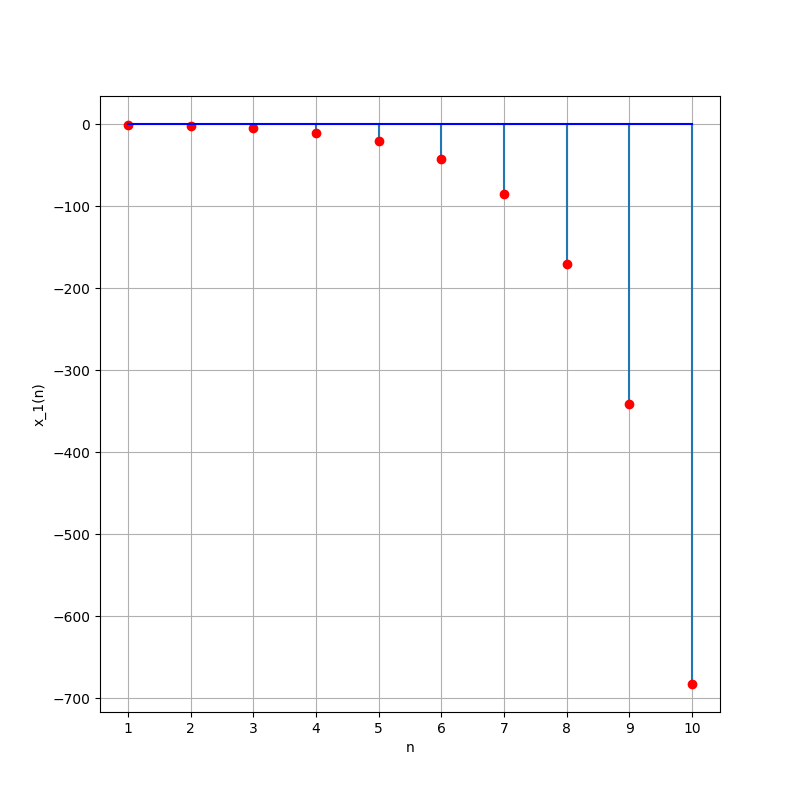
\includegraphics[width=1.0\columnwidth]{ncert-maths/11/9/3/16/figs/plot1.png}
  \caption{Representation of x(n) for $r=2$}
  \label{fig:fig1}
\end{figure}
\begin{figure}[h]
  \centering
  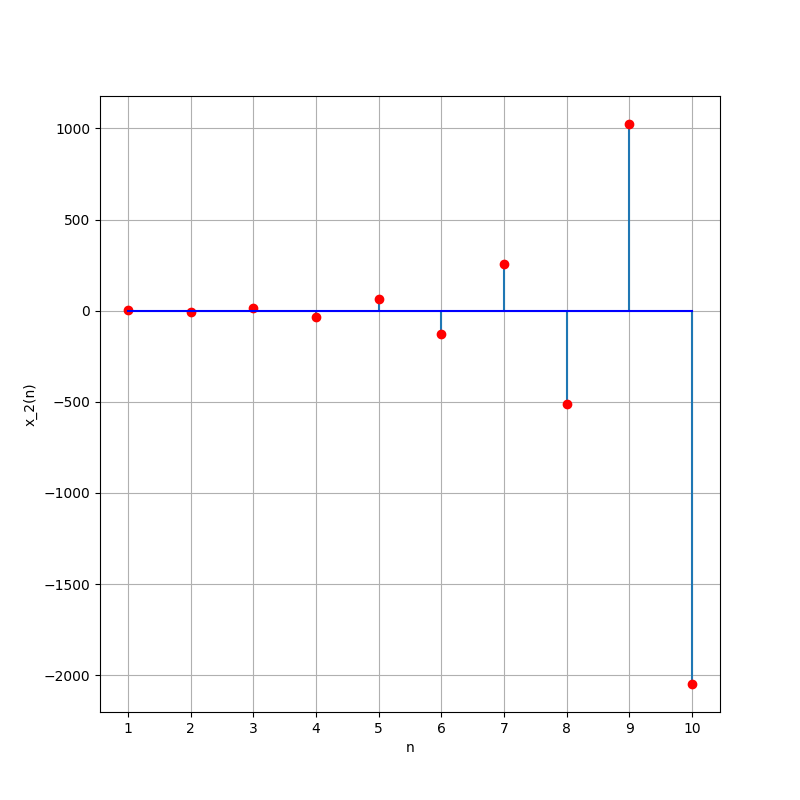
\includegraphics[width=1.0\columnwidth]{ncert-maths/11/9/3/16/figs/plot2.png}
  \caption{Representation of x(n) for $r=-2$}
  \label{fig:fig2}
\end{figure}


%\end{document}

\pagebreak

\item Find the sum of the following series up to n terms and obtain the Z-transform: 
$$\ldots + 0 + \frac{1^3}{1} + \frac{1^3 + 2^3}{1 + 3} + \frac{1^3 + 2^3 + 3^3}{1 + 3 + 5} + \ldots$$
\solution
\pagebreak
\item Insert five numbers between 8 and 26 such that the resulting sequence is an A.P. and obtain the Z-transform of the sequence.
\pagebreak

\item If \(S_1\), \(S_2\), \(S_3\) are the sum of the first \(n\) natural numbers, their squares, and their cubes, respectively, show that 
\[ 9(S_2)^2 = (S_3)(1 + 8(S_1)) \]\\
\solution
\pagebreak


\item If a, b, c, d are in G.P, prove that 
$ \brak{a^{n} + b^{n}},\brak{b^{n} + c^{n}},\brak{c^{n} + d^{n}} $ are in G.P \\
\solution
\iffalse
\let\negmedspace\undefined
\let\negthickspace\undefined
\documentclass[journal,12pt,twocolumn]{IEEEtran}
\usepackage{cite}
\usepackage{amsmath,amssymb,amsfonts,amsthm}
\usepackage{algorithmic}
\usepackage{graphicx}
\usepackage{textcomp}
\usepackage{xcolor}
\usepackage{txfonts}
\usepackage{listings}
\usepackage{enumitem}
\usepackage{mathtools}
\usepackage{gensymb}
\usepackage{comment}
\usepackage[breaklinks=true]{adjustbox}
\usepackage{tkz-euclide} 
\usepackage{listings}
\usepackage{gvv}                                        
\def\inputGnumericTable{}                                 
\usepackage[latin1]{inputenc}                                
\usepackage{color}                                            
\usepackage{array}                                            
\usepackage{longtable}                                       
\usepackage{calc}                                             
\usepackage{multirow}                                         
\usepackage{hhline}                                           
\usepackage{ifthen}                                           
\usepackage{lscape}

\newtheorem{theorem}{Theorem}[section]
\newtheorem{problem}{Problem}
\newtheorem{proposition}{Proposition}[section]
\newtheorem{lemma}{Lemma}[section]
\newtheorem{corollary}[theorem]{Corollary}
\newtheorem{example}{Example}[section]
\newtheorem{definition}[problem]{Definition}
\newcommand{\BEQA}{\begin{eqnarray}}
\newcommand{\EEQA}{\end{eqnarray}}
\newcommand{\define}{\stackrel{\triangle}{=}}
\theoremstyle{remark}
\newtheorem{rem}{Remark}

\begin{document}
\bibliographystyle{IEEEtran}

\vspace{3cm}

\title{}
\author{EE23BTECH11047 - Deepakreddy P
}
\maketitle

\noindent \textbf{17} \quad 
If a, b, c, d are in G.P, prove that 
$ \brak{a^{n} + b^{n}},\brak{b^{n} + c^{n}},\brak{c^{n} + d^{n}} $ are in G.P \\
\solution
\fi


\begin{center}
    \begin{table}[ht]
        \setlength{\arrayrulewidth}{0.3mm}
\setlength{\tabcolsep}{12pt}
\renewcommand{\arraystretch}{1.5}


\begin{center}
\caption{Input Parameters}
\begin{tabular}{|c|c|}

\hline
 {Symbol}&{Remarks}\\
\hline
$x(0) $ & $a$ \\
\hline
$x(1) $ & $b$ \\
\hline
$x(2) $ & $c$ \\
\hline
$x(3) $ & $d$ \\
\hline
$r$ & ratio of G.P a,b,c....\\
\hline
$r_1$ & ratio of G.P $a^n + b^n,b^n + c^n,....$\\
\hline
$X(z)$ & z transform of G.P a,b,c....\\
\hline
$Y(z)$ & z transform of G.P $a^n + b^n,b^n + c^n,....$\\
\hline

\end{tabular}
\label{Table:11.9.5.17.3}
\end{center}

    \end{table}
\end{center}

From \tabref{Table:11.9.5.17.3}

\begin{align}   
r=\frac{b}{a} = \frac{c}{b}= \frac{d}{c} \label{eq:eq.11.9.5.17.1}
\end{align}

From eq \eqref{eq:eq.11.9.5.17.1}

\begin{align}
\frac{b^n + c^n}{a^n + b^n}
&= \frac{\brak{ar}^n + \brak{ar^2}^n}{\brak{a}^n + \brak{ar}^n}\\
&= \frac{a^n r^n \brak{1+ r^n}}{a^n \brak{1 + r^n}}\\
&= r^n \\
\frac{c^n + d^n}{b^n + c^n}&= \frac{\brak{ar^2}^n + \brak{ar^3}^n}{\brak{ar}^n + \brak{ar^2}^n}\\
&= \frac{a^n r^{2n} \brak{1 + r^n}}{a^n r^n \brak{1 + r^n}}\\
%&= \frac{r^n \brak{\brak{ar}^n + \brak{ar^2}^n}}{r^n \brak{\brak{a}^n + \brak{ar}^n}}
&= r^n \\
\frac{b^n + c^n}{a^n + b^n} &= \frac{c^n + d^n}{b^n + c^n}
\end{align}
Hence proved they are in in G.P\\

\begin{align}
    x\brak{n} &= a\brak{\frac{b}{a}}^{n} u\brak{n}\\
    X\brak{z} &= \frac{a}{1-\brak{\frac{b}{a}} z^{-1}}, \quad \abs{z}>\abs{\frac{b}{a}}
\end{align}

\begin{align}   
r_1=\frac{b^n + c^n}{a^n + b^n} = \frac{c^n + d^n}{b^n + c^n} \label{eq:eq.11.9.5.17.2}
\end{align}

From eq \eqref{eq:eq.11.9.5.17.2}

\begin{align}
    y\brak{n} &= \brak{a^n + b^n} \brak{\frac{b^n + c^n}{a^n + b^n}}^{n} u\brak{n}\\
    Y\brak{z} &= \frac{a^n + b^n}{1-\brak{\frac{b^n + c^n}{a^n + b^n}} z^{-1}}, \quad \abs{z}>\abs{\frac{b^n + c^n}{a^n + b^n}}
\end{align}


\begin{figure}[ht]
   \centering
   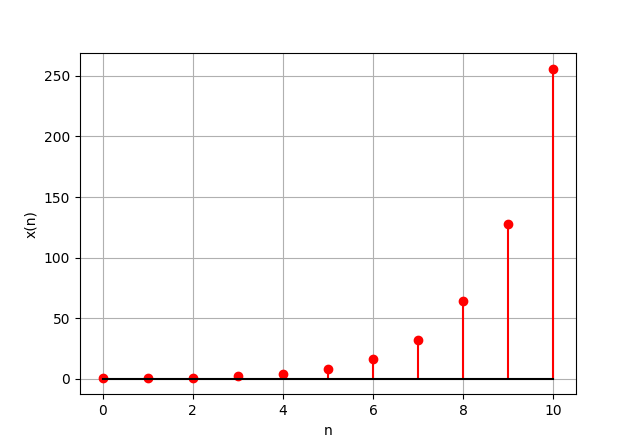
\includegraphics[width=0.8\columnwidth]{ncert-maths/11/9/5/17/figs/gp1.png}
   \caption{Stem Plot of $x(n) = (0.25) 2^n u(n)$, $a= 0.25, r=2$}
\end{figure}

\begin{figure}[ht]
   \centering
   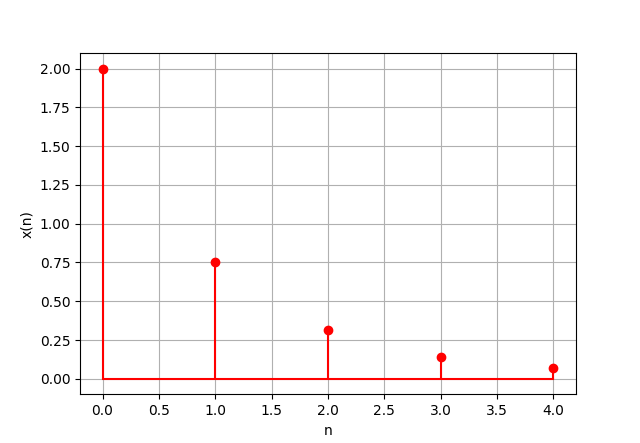
\includegraphics[width=0.8\columnwidth]{ncert-maths/11/9/5/17/figs/gp2.png}
   \caption{Stem Plot of $x(n) = \brak{0.25^n + 0.5^n} u(n)$, $a=0.25, b=0.5$}
\end{figure}

%\end{document}

\pagebreak
\item Write the first five terms of the sequence whose $n^{th}$ terms  $x\brak{n} = \frac{n}{n+1}$\\
\solution
\pagebreak
\item 150 workers were engaged to finish a job in a certain number of days, 4 workers dropped out on second day, 4 more workers dropped out on third day and so on. It took 8 more days to finish the work. Find the number of days in which the work was completed.\\
\solution
\pagebreak

\item The Fibonacci sequence is defined by 1 = a$1$ = a$_2$ and a$_n$ = a${n-1}$ + a$_{n-2}$ , n $\textgreater$ 2\\
Find $\dfrac{a_{n + 1}}{a_n}$, for n = 1, 2, 3, 4, 5\\
\solution
\pagebreak

\item  A farmer buys a used tractor for Rs 12000. He pays Rs 6000 in cash and agrees to pay the balance in annual installments of Rs 500 plus 12 \% interest on the unpaid amount. How much will the tractor cost him?
\solution
\pagebreak

\item 1) Find the sum to n terms for the given series: $3\times8 + 6\times11 + 9\times14 + ...$
\solution
\pagebreak

\item The sum of the first $n$ terms of two arithmetic progressions (AP) is in the ratio $5n+4 : 9n+6$. Find the ratio of their 18th terms.\\
\solution
\pagebreak

\item How many terms of the AP : 9, 17, 25, . . . must be taken to give a sum of 636?
\solution
\pagebreak

\item Find the sum to indicated number of terms in the geometric progression:\\
1, $– a$, $a^2$
, $-a^3$
, ... n terms (if $a \neq – 1$).\\
\solution
\pagebreak

\end{enumerate}
